\pdfoutput=1
\documentclass[11pt,letterpaper,twoside,reqno,nosumlimits]{amsart}
\usepackage{graphicx}
\usepackage{amssymb,bm} % for some reason, also had mathbbol
\usepackage{enumerate,setspace}
\usepackage{hyperref}

\evensidemargin=0in
\oddsidemargin=0in
\textwidth=6.5in
\topmargin=-0.33in
\headheight=0.25in
\textheight=9in

% this one is my bad: I need to go through and manually convert all the stars to asterisks, but for now, taking a shortcut
\renewcommand{\star}{*}

\newcommand{\mat}[1]{\ensuremath{\bm{#1}}} % can also use mathbf, but then matrices appear upright instead of slanted
\renewcommand{\vec}[1]{\ensuremath{\bm{#1}}}
\newcommand{\e}{\ensuremath{\mathrm{e}}}
\newcommand{\E}{\ensuremath{\mathbb{E}}}
\newcommand{\Prob}[1]{\ensuremath{\mathbb{P}\left\{#1\right\}}}
\newcommand{\lnorm}[2]{\ensuremath{\left\| #2 \right\|_{#1}}}
\newcommand{\R}{\ensuremath{\mathbb{R}}}
\newcommand{\C}{\ensuremath{\mathbb{C}}}
\newcommand{\randcon}{\ensuremath{\Psi}}
\newcommand{\s}{s} % singular values

\newcommand{\norm}[1]{\ensuremath{\left\|#1\right\|}}
\newcommand{\snorm}[1]{\ensuremath{\|#1\|}}
\newcommand{\lambdamax}[1]{\ensuremath{\lambda_{\mathrm{max}}\left(#1\right)}}
\newcommand{\lambdamin}[1]{\ensuremath{\lambda_{\mathrm{min}}\left(#1\right)}}
\newcommand{\Isom}[2]{\ensuremath{\mathbb{V}_{#1}^{#2}}}
\newcommand{\samats}[1]{\ensuremath{\mathbb{M}^{#1}_{\mathrm{sa}}}}
\DeclareMathOperator{\tr}{tr}
\DeclareMathOperator{\rank}{rank}
\newcommand{\trexp}[1]{\ensuremath{\tr\exp\left\{#1\right\}}}

% Change definition of cases environment to allow adding an optional arraystretch param
% e.g. \begin{cases}[0.8] ... \end{cases}
\makeatletter
\renewcommand*\env@cases[1][1.2]{%
  \let\@ifnextchar\new@ifnextchar
  \left\lbrace
  \def\arraystretch{#1}%
  \array{@{}l@{\quad}l@{}}%
}
\makeatother

% GET MACRO FILE FROM JOEL, SEE NUMBERWITHIN TO NUMBER STUFF BY SECTION
\newtheorem{thm}{Theorem}
\newtheorem{prop}{Proposition}
\newtheorem{lemma}[thm]{Lemma}
\newtheorem{cor}[thm]{Corollary}
\newtheorem{defn}{Definition}
\theoremstyle{remark}
\newtheorem{remark}{Remark}

\numberwithin{equation}{section}
\numberwithin{thm}{section}
\numberwithin{prop}{section}
\numberwithin{defn}{section}
\numberwithin{remark}{section}

\title[Tail Bounds for Eigenvalues of Random Matrices]{Tail Bounds for All Eigenvalues \\ of A Sum of Random Matrices}
\date{April 8, 2011}
\author[A.~Gittens]{Alex~Gittens}
%\email{gittens@cms.caltech.edu}
\author[J.~A.~Tropp]{Joel~A.~Tropp}
%\email{jtropp@cms.caltech.edu}
\thanks{Both authors can be reached at Annenberg Center, MC 305-16, California Institute of Technology, 1200 E. California Blvd., Pasadena, CA 91125. Email: {\tt gittens@cms.caltech.edu} and {\tt jtropp@cms.caltech.edu}. Research supported by ONR awards N00014-08-1-0883 and N00014-11-1-0025, AFOSR award FA9550-09-1-0643, and a Sloan Fellowship.}
%\subjclass{}
%\keywords{}

\begin{document}
\begin{abstract}
This work introduces the minimax Laplace transform method, a modification of the cumulant-based matrix Laplace transform method developed in \cite{T10a} that yields \emph{both} upper and lower bounds on \emph{each} eigenvalue of a sum of random self-adjoint matrices. This machinery is used to derive eigenvalue analogues of the classical Chernoff, Bennett, and Bernstein bounds.
%This work introduces a straightforward minimax method for extending bounds on the largest and smallest eigenvalues of random self-adjoint matrices into bounds on each eigenvalue. Merging this with the matrix Laplace transform framework established in \cite{T10a} produces a minimax Laplace transform which allows one to reproduce versions of classical bounds for each eigenvalue of a sum of random self-adjoint matrices. The paper demonstrates the derivation of Chernoff, Bennett, and Bernstein eigenvalue bounds through the minimax Laplace transform. 

Two examples demonstrate the efficacy of the minimax Laplace transform. The first concerns the effects of column sparsification on the spectrum of a matrix with orthonormal rows. Here, the behavior of the singular values can be described in terms of coherence-like quantities. The second example addresses the question of relative accuracy in the estimation of eigenvalues of the covariance matrix of a random process. Standard results on the convergence of sample covariance matrices provide bounds on the number of samples needed to obtain relative accuracy in the spectral norm, but these results only guarantee relative accuracy in the estimate of the maximum eigenvalue. The minimax Laplace transform argument establishes that $\Omega(\varepsilon^{-2} p \log p)$ samples are sufficient to ensure that \emph{all} the eigenvalues of the covariance matrix of a $\mathcal{N}(\vec{0}, \mat{C})$ random vector are estimated to within a factor of $1 \pm \varepsilon$ with high probability.


%To illustrate the efficacy of the minimax method, it is used to investigate the rate of convergence, in relative error, of each eigenvalue of the empirical covariance matrix associated with a Gaussian random vector. It results that one needs at most $\mathrm{O}((p \log p)/\epsilon^2)$ observations to estimate the full spectrum of the covariance matrix to within $(1 \pm \epsilon)$ relative error with constant probability. The Chernoff bounds are also used to determine the effect of column sparsification on the spectra of wide matrices with orthonormal rows. 
\end{abstract}

\maketitle

%\doublespacing
\section{Introduction}
In this paper, we introduce a simple method, based upon the variational characterization of eigenvalues, that parlays bounds on the extreme eigenvalues of sums of random self-adjoint matrices into bounds that apply to all the eigenvalues. This technique fits snugly into the matrix Laplace transform method detailed in \cite{T10a}. We combine these ideas to extend several of the inequalities in \cite{T10a} to address the fluctuations of interior eigenvalues. 

As one application of our approach, we investigate estimates for the covariance matrix of a centered stationary random process. We show that the eigenvalues of the sample covariance matrix provide relative-error approximations to the eigenvalues of the covariance matrix. We focus on Gaussian processes, but our arguments can be extended to other distributions. The following theorem is a distillation of the results in section \ref{sec:covarianceest}.
\begin{thm}
Assume $\mat{C}$ is positive semidefinite. Let $\{\vec{\eta}_j\}_{j=1}^n \subset \R^p$ be i.i.d. samples drawn from a $\mathcal{N}(\vec{0}, \mat{C})$ distribution. Define the sample covariance matrix
\[
\widehat{\mat{C}}_n = \frac{1}{n} \sum\nolimits_{j=1}^n \vec{\eta}_j\vec{\eta}_j^\star.
\]
If $n = \Omega(\varepsilon^{-2} p \log p),$ then with high probability
\[
|\lambda_k(\widehat{\mat{C}}_n) - \lambda_k(\mat{C})| \leq \varepsilon \lambda_k(\mat{C}) \quad \text{for } k=1, \ldots,p.
\]
\label{thm:examplecovarest}
\end{thm}
Thus, $n = \mathrm{K} \varepsilon^{-2} p \log p$ samples suffice to ensure that all of the eigenvalues of $\mat{C}$ are captured to relative precision $1 \pm \varepsilon.$ This estimate can be sharpened, given the spectrum of $\mat{C}$ and the desired failure probability. The same tools can be used to estimate $\lambda_k(\widehat{\mat{C}}_n - \mat{C}).$

\subsection{Related Work}

Theorem \ref{thm:examplecovarest} provides information about the entire spectrum of a random matrix, including the limiting behavior of the eigenvalues and a bound on the rate at which they converge. We believe that this paper contains the first general-purpose tools for studying the full spectrum of a finite-dimensional random matrix. The literature on random matrix theory (RMT) contains some complementary results, but they do not seem to apply with the same generality. Methods from RMT fall into two rough categories: asymptotic methods and nonasymptotic methods. We discuss the relevant results from each in turn.

The modern asymptotic theory began in the 1950s with the observation by physicists that, on certain scales, the behavior of quantum systems is described by the spectra of random matrices. They further observed the phenomenon of \emph{universality}: as the dimension increases, the statistics of their spectra become largely independent of the particular choice of distribution the random matrices are drawn from. Since this time, physicists, statisticians, engineers, and mathematicians have found manifold applications of the asymptotic theory in large-dimensional statistics, physics, wireless communication, and pure mathematics, to mention only a few areas. 

Asymptotic random matrix theory has developed primarily through the study of sample covariance matrices and \emph{ensembles}, certain classes of random matrices. The most studied ensembles are the various Wigner ensembles, consisting of Hermitian matrices whose entries are i.i.d. up to the constraints imposed by the symmetry condition. To state the fundamental result on Wigner ensembles, we introduce the empirical spectral distribution function (ESD) of a Hermitian matrix $\mat{A}$,
\[
F^{\mat{A}}(x) = \frac{1}{n} \#\{ 1 \leq i \leq n : \lambda_i(\mat{A}) \leq x \}.
\]
We see that $F^{\mat{A}}$ is a random measure that encodes the statistics of the spectrum of $\mat{A}.$ Wigner's theorem, the seminal result in the asymptotic theory, establishes that the ESD of the Wigner ensemble consisting of matrices whose entries are i.i.d $\mathcal{N}(0, 1/n)$ random variables converges, as $n$ approaches infinity, to the semicircular law, given by 
\[
F(x) = \begin{cases}
\frac{1}{2\pi}\sqrt{4 - x^2}, & \text{if } |x| \leq 2, \\
0 & \text{otherwise.}
\end{cases}
\] 
Thus, at least in the limiting sense, the spectrum of an element drawn from this ensemble is well characterized. The development of the classical asymptotic theory has been driven by the natural question raised by Wigner's result: to what extent is the semicircular law, or more generally, the existence of a limiting spectral distribution universal?

Ony recently has the tide of research turned towards questions more germane to our specific concerns. the speed of the convergence of ESDs and the deviations of eigenvalues from the positions implied by the limiting spectral distributions.

The current paper is ultimately based on the influential work of Ahlswede and Winter~\cite{AW02}. This line of  research leads to explicit tail bounds for the maximum eigenvalue of a sum of random matrices. These probability inequalities parallel the classical scalar tail bounds due to Bernstein and others. Matrix probability inequalities are interesting because they allow us to obtain valuable information about the maximum eigenvalue of a random matrix with very little effort. Furthermore, they apply to a wide variety of random matrices. On the other hand, this approach does not always yield sharp results because parasitic logarithmic factors arise in many settings.

%Random matrices are employed in an increasing number of applications; to mention just a few: machine learning \cite{D04}, robust convex optimization \cite{So09,Nem07}, approximation algorithms for NP hard optimization problems \cite{Tamas06,So09b,FPR10}, and fast computational linear algebra \cite{HMT09,B09}. In each of these areas, the feasibility and efficacy of randomized algorithms is determined by the spectra of the random matrices used. 

%Classical asymptotic random matrix theory tools--- method of moments and Stieltjes transforms--- can be used to obtain results which describe, for certain ensembles of random matrices, the limit of the spectral distributions as the matrix size approaches infinity \cite{Bai99,BS06}. Unfortunately, these results address the convergence of the empirical spectral distributions and the extreme eigenvalues, not that of the interior eigenvalues. Furthermore, the m\'etier of these techniques is the determination of convergence, rather than the development of tail bounds which hold at a fixed dimension. To develop such bounds, we turn to the complementary field of nonasymptotic random matrix theory.

%In addition to providing quantitative bounds on the extreme eigenvalues of random matrices of fixed dimensions, the tools of nonasymptotic random matrix theory apply to a wider class of matrices than those of asymptotic random matrix theory. For instance, the $\varepsilon$-net technique applies to random matrices with independent elements that exhibit sufficiently strong tail decay \cite{Ver10, DNT10}. To bound the extreme eigenvalues of a sum of fixed matrices with random signs, one can use the noncommutative Khintchine inequality, or if the summands are rank-one and symmetric, a lemma due to Rudelson; these require only bounds on the maximum singular values of the summands \cite{So09,RU99}. Using symmetrization and decoupling arguments, these two techniques can be used to bound the extreme eigenvalues of even more general random matrices \cite{RV07}. Perhaps the most generally applicable tool in the arsenal of nonasymptotic random matrix theory is the matrix Laplace transform technique pioneered by Ahlswede and Winter, which applies to sums of independent random matrices \cite{AW02,T10a}.

%Even in the case of Wishart matrices, where the spectral distribution is known exactly, extracting quantitative bounds on the behavior of the interior eigenvalues is a nontrivial task. Thus it is no surprise that the standard tools of nonasymptotic random matrix theory---the noncommutative Khintchine inequality \cite{So09}, a lemma due to Rudelson \cite{RU99}, the approach of Ahlswede and Winter \cite{AW02}, and $\varepsilon$-net arguments \cite{Ver10} possibly augmented with the entropy-concentration tradeoff \cite{DNT10}---give one information on only the largest and smallest eigenvalues. Instead, it is surprising that the bounds on the extreme eigenvalues one obtains using these tools can be quite sharp.

%Despite their flexibility, and the fact that they provide (sometimes quite sharp) bounds for random matrices of fixed dimensions, the available frameworks for nonasymptotic random matrix theory are still limited in scope. Specifically, they provide results applicable only to the extreme eigenvalues and generally bound the deviations in only one direction. Thus, we may control the probability that the largest eigenvalue is exceptionally large, but have no control over the probability that it is exceptionally small. %To date there has been no general framework for quantitatively addressing questions about the fluctuations of interior eigenvalues of random matrices. 
%In this work, we address these deficiencies by using the Laplace transform machinery to develop a framework for quantitatively addressing questions about the fluctuations, in both directions,  of each eigenvalue of a sum of independent random matrices.

\subsection{Outline}
In section \ref{sec:background}, we introduce the notation used in this paper and state a convenient version of the Courant--Fischer theorem. In section \ref{sec:laplacetransform}, we use the Courant--Fischer theorem to extend the Laplace transform technique from \cite{T10a} to apply to all the eigenvalues of self-adjoint matrices, thereby obtaining the minimax Laplace transform. We apply this technique in sections \ref{sec:chernoffbounds} and \ref{sec:bernsteinbounds} to develop eigenvalue analogues of the classical Chernoff and Bernstein bounds. The final two sections illustrate, using two familiar problems, that the minimax Laplace technique gives us significantly more information on the spectra of random matrices than current approaches. In section \ref{sec:colsubsampling}, we use the Chernoff bounds to quantify the effects of column sparsification on all the singular values of matrices with orthogonal rows. In section \ref{sec:covarianceest}, we consider the question of how fast, in relative error, the eigenvalues of empirical covariance matrices converge.

\section{Background and Notation}
\label{sec:background}
We establish the notation used in the sequel and state a convenient version of the Courant--Fischer theorem.

Unless otherwise stated, we work over the complex field. The $k$th column of the matrix $\mat{A}$ is denoted by $\mat{a}_k,$ and the entries are denoted $a_{jk}$ or $(\mat{A})_{jk}.$ We define $\samats{n}$ to be the set of self-adjoint matrices with dimension $n.$ The eigenvalues of a matrix $\mat{A}$ in $\samats{n}$ are arranged in weakly decreasing order: $\lambdamax{\mat{A}} = \lambda_1(\mat{A}) \geq \lambda_2(\mat{A}) \geq \cdots \geq \lambda_n(\mat{A}) = \lambdamin{\mat{A}}.$ Likewise, singular values of a rectangular matrix $\mat{B}$ with rank $r$ are ordered $\s_1(\mat{B}) \geq \s_2(\mat{B}) \geq \cdots \geq \s_r(\mat{B}).$ The spectral norm of a matrix $\mat{B}$ is expressed as $\snorm{\mat{B}}.$ We often compare self-adjoint matrices using the semidefinite ordering. In this ordering, $\mat{A}$ is greater than or equal to $\mat{B}$, written $\mat{A} \succeq \mat{B}$ or $\mat{B} \preceq \mat{A},$ when $\mat{A} - \mat{B}$ is positive semidefinite.

The expectation of a random variable is denoted by $\E X.$ We write $X \sim \text{Bern}(p)$ to indicate that $X$ has a Bernoulli distribution with mean $p.$

One of our central tools is the variational characterization of the eigenvalues of a self-adjoint matrix given by the Courant--Fischer theorem. 
For integers $d$ and $n$ satisfying $1 \leq d \leq n$, the complex Stiefel manifold 
\[
\Isom{d}{n} = \{\mat{V} \in \C^{n \times d} \,:\, \mat{V}^\star \mat{V} = \mathbf{I} \}
\]
is the collection of orthonormal bases for the $d$-dimensional subspaces of $\C^n,$ or, equivalently, the collection of all isometric embeddings of $\C^d$ into $\C^n.$ Let $\mat{A}$ be a self-adjoint matrix with dimension $n,$ and let $\mat{V} \in \Isom{d}{n}$ be an orthonormal basis for a subspace of $\C^n.$ Then the matrix $\mat{V}^\star \mat{A} \mat{V}$ can be interpreted as the compression of $\mat{A}$ to the space spanned by $\mat{V}.$

\begin{prop}[Courant--Fischer]
\label{prop:isometrycf}
Let $\mat{A}$ be a self-adjoint matrix with dimension $n$. Then
\begin{align}
\lambda_k(\mat{A}) & = \min_{\mat{V} \in \Isom{n-k+1}{n}} \lambdamax{\mat{V}^\star\mat{AV}} \quad \text{and}
\label{eqn:maxvariation} \\
\lambda_k(\mat{A}) & = \max_{\mat{V} \in \Isom{k}{n}} \lambdamin{\mat{V}^\star \mat{AV}}. \label{eqn:minvariation}
\end{align}
A matrix $\mat{V}_- \in \Isom{k}{n}$ achieves equality in~\eqref{eqn:minvariation} if and only if its columns span a dominant $k$-dimensional invariant subspace of $\mat{A}.$ Likewise, a matrix $\mat{V}_+ \in \Isom{n-k+1}{n}$ achieves equality in~\eqref{eqn:maxvariation} if and only if its columns span a bottom $(n-k+1)$-dimensional invariant subspace of $\mat{A}$.
\end{prop}

The $\pm$ subscripts in Proposition \ref{prop:isometrycf} are chosen to reflect the fact that $\lambda_k(\mat{A})$ is the \emph{minimum} eigenvalue of $\mat{V}_-^\star\mat{A}\mat{V}_-$ and the \emph{maximum} eigenvalue of $\mat{V}_+^\star \mat{A} \mat{V}_+.$ 
As a consequence of Proposition \ref{prop:isometrycf}, when $\mat{A}$ is self-adjoint, \mbox{$\lambda_k(-\mat{A}) = -\lambda_{n-k+1}(\mat{A}).$} This fact allows us to use the same techniques we develop for bounding the eigenvalues from above to bound them from below.

\section{ Tail Bounds For Interior Eigenvalues}
\label{sec:laplacetransform}
In this section we develop a generic bound on the tail probabilities of eigenvalues of sums of independent, random, self-adjoint matrices. We establish this bound by supplementing the matrix Laplace transform methodology of \cite{T10a} with Proposition \ref{prop:isometrycf} and a new result, due to Lieb and Seiringer \cite{LS05}, on the concavity of a certain trace function on the cone of positive-definite matrices.

 First we observe that the Courant--Fischer theorem allows us relate the behavior of the $k$th eigenvalue of a matrix to the behavior of the largest eigenvalue of an appropriate compression of the matrix.
% NOTE:
% PINCHING -> removes interactions between subspaces
% COMPRESSION -> removes all but one subspace


% MAYBE USE A Y IN THIS STATEMENT OF THEM TO AVOID CONFUSION WHEN X = SUM X_j LATER
\begin{thm}
Let $\mat{X}$ be a random self-adjoint matrix with dimension $n,$ and let $k \leq n$ be an integer. Then, for all $t \in \R,$
\begin{equation}
\Prob{\lambda_k(\mat{X}) \geq t} \leq \inf_{\theta > 0} \min_{\mat{V} \in \Isom{n-k+1}{n}} \left\{ \e^{-\theta t} \cdot \E\tr\e^{\theta \mat{V}^\star\mat{XV}} \right\}.
\label{eqn:laplacetform}
\end{equation}
\label{thm:laplacetform}
\end{thm}

% JOEL PREFERS BRACES FOR EXPONENTIAL, AND USE BIG BIGG ETC TO FINER CONTROL THEIR SIZES
\begin{proof}
Let $\theta$ be a fixed positive number. Then
\begin{multline*}
\Prob{\lambda_k(\mat{X}) \geq t}  = 
\Prob{\lambda_k(\theta \mat{X}) \geq \theta t} = 
\Prob{\e^{\lambda_k(\theta \mat{X})} \geq \e^{\theta t}} \\
\leq  \e^{-\theta t} \cdot \E \e^{\lambda_k(\theta \mat{X})} = 
\e^{-\theta t} \cdot \E \exp\left\{\min_{\mat{V} \in \Isom{n-k+1}{n}} \lambdamax{\theta \mat{V}^\star\mat{XV}}\right\}. 
\end{multline*}
The first identity follows from the positive homogeneity of eigenvalue maps and the second from the monotonicity of the scalar exponential function. The final two relations are Markov's inequality and \eqref{eqn:maxvariation}.

To continue, we need to bound the expectation. Interchange the order of the exponential and the minimum; then apply the spectral mapping theorem to see that
\begin{align*}
 \E \exp\bigg\{\min_{\mat{V} \in \Isom{n-k+1}{n}} \lambdamax{\theta \mat{V}^\star \mat{XV}} \bigg\} & = \E \min_{\mat{V} \in \Isom{n-k+1}{n}} \lambdamax{\exp(\theta \mat{V}^\star\mat{XV})} \\
  & \leq \min_{\mat{V} \in \Isom{n-k+1}{n}} \E \lambdamax{\exp(\theta \mat{V}^\star\mat{XV})} \\
  & \leq \min_{\mat{V} \in \Isom{n-k+1}{n}} \E \tr \exp(\theta \mat{V}^\star\mat{XV}).
\end{align*}
The first inequality is Jensen's. The second inequality follows because the exponential of a self-adjoint matrix is positive definite, so its largest eigenvalue is smaller than its trace.

Combine these observations and take the infimum over all positive $\theta$ to complete the argument.
\end{proof}

We are interested in the case where the matrix $\mat{X}$ in Theorem \ref{thm:laplacetform} can be expressed as a sum of independent random matrices. In this case, we use the following result to develop the right-hand side of the Laplace transform bound \eqref{eqn:laplacetform}.

% In most cases it is prohibitively difficult to directly estimate the quantity $\E \tr \e^{\theta \mat{V}^\star\mat{XV}}.$ The main contribution of \cite{T10a} is a bound on this quantity, when $\mat{V} = \mathbf{I}$, in terms of the cumulant generating functions of the summands. The main tool in the proof is a classical result due to Lieb \cite{Lieb1973} that establishes the concavity of the function
% \begin{equation}
% \mat{A} \mapsto \trexp{\mat{H} + \log(\mat{A})}, \quad \text{ where $\mat{H}$ is self-adjoint} \label{eqn:tracefunctional}
% \end{equation}
% on the positive definite cone.

% The next result gives a similar bound on $\E \trexp{\theta \mat{V}^\star \mat{X}\mat{V}}$ in the case of general isometric embeddings $\mat{V}.$

\begin{thm}
Consider a finite sequence $\{\mat{X}_j\}$ of independent, random, self-adjoint matrices with dimension $n$ and a sequence $\{\mat{A}_j\}$ of fixed self-adjoint matrices with dimension $n$ that satisfy the relations
\begin{equation}
 \E\e^{\mat{X}_j} \preceq \e^{\mat{A}_j}. 
 \label{eqn:logmgfdomination}
\end{equation}
Let $\mat{V} \in \Isom{k}{n}$ be an isometric embedding of $\C^k$ into $\C^n$ for some $k \leq n.$ Then
\begin{equation}
 \E \tr \exp\left\{\sum\nolimits_j \mat{V}^\star \mat{X}_j \mat{V} \right\} \leq \tr \exp\left\{\sum\nolimits_j \mat{V}^\star \mat{A}_j \mat{V} \right\}.
 \label{eqn:pinchedmgf}
\end{equation}
In particular, 
\begin{equation}
 \E \tr \exp\left\{\sum\nolimits_j \mat{X}_j \right\} \leq \tr \exp\left\{\sum\nolimits_j \mat{A}_j \right\}.
 \label{eqn:unpinchedmgf}
\end{equation}

\label{thm:mgf}
\end{thm}

%\begin{remark}
 %Since the matrix exponential is operator monotone and the matrix logarithm is operator monotone on $(0, \infty),$ the condition
%\[
% \E\e^{\mat{X}_j} \preceq \e^{\mat{A}_j}
%\]
%is satisfied if and only if it is also the case that 
%\[ 
%  \log \left( \E\e^{\mat{X}_j} \right) \preceq \mat{A}_j. 
%\]

%Because of this latter relation, we call $\mat{A}_j$ a semidefinite bound on the cumulant generating function of $\mat{X}_j.$
%\end{remark}

%Tropp's original bound on the moment generating function is an immediate corollary of Theorem \ref{thm:mgf}. 

%\begin{cor}
% Consider a finite sequence $\{\mat{X}_j\}$ of independent, random, self-adjoint matrices and a sequence $\{\mat{A}_j\}$ of fixed self-adjoint %matrices that satisfy the relations
%\begin{equation*}
% \E\e^{\mat{X}_j} \preceq \e^{\mat{A}_j}.
%\end{equation*}
%Then
%\[
%  \E \trexp{\sum\nolimits_j \mat{X}_j } \leq \trexp{\sum \mat{A}_j}. 
% \]
% \label{cor:troppmgf}
% \end{cor}

Theorem \ref{thm:mgf} is an extension of Lemma 3.4 of \cite{T10a}, which establishes the special case \eqref{eqn:unpinchedmgf}. The proof depends upon a recent result due to Lieb and Seiringer \cite[Thm.~3]{LS05} that extends Lieb's earlier result \cite[Thm.~6]{Lieb1973}.

\begin{prop}[Lieb--Seiringer 2005]
Let $\mat{H}$ be a self-adjoint matrix with dimension $k.$ Let $\mat{V} \in \Isom{k}{n}$ be an isometric embedding of $\C^k$ into $\C^n$ for some $k \leq n.$ Then the function
\begin{equation*}
 \mat{A} \longmapsto \trexp{\mat{H} + \mat{V}^\star (\log\mat{A}) \mat{V}}
\end{equation*}
is concave on the cone of positive-definite matrices in \samats{n}.
 \label{prop:pinchedtracefunctional}
\end{prop}

\begin{proof}[Proof of Theorem \ref{thm:mgf}]
 First, note that \eqref{eqn:logmgfdomination} and the operator monotonicity of the matrix logarithm yield the following inequality for each $k$: 
\begin{equation}
\log \E \e^{\mat{X}_k} \preceq \mat{A}_k.
\label{eqn:logdom}
\end{equation}
Let $\E_k$ denote expectation conditioned on the first $k$ summands, $\mat{X}_1$ through $\mat{X}_k.$ Then
\begin{align*}
 \E \trexp{\sum_{j \leq \ell} \mat{V}^\star \mat{X}_j \mat{V}} & = \E\E_1\cdots \E_\ell \trexp{\sum_{j \leq \ell-1} \mat{V}^\star \mat{X}_j \mat{V} + \mat{V}^\star \left( \log \e^{\mat{X}_\ell} \right) \mat{V}} \\
 & \leq \E\E_1\cdots \E_{\ell-1} \trexp{\sum_{j \leq \ell-1} \mat{V}^\star \mat{X}_j \mat{V} + \mat{V}^\star \left( \log\E\e^{\mat{X}_\ell} \right) \mat{V}} \\
 & \leq \E\E_1\cdots \E_{\ell-1} \trexp{\sum_{j \leq \ell-1} \mat{V}^\star \mat{X}_j \mat{V} + \mat{V}^\star \left( \log\e^{\mat{A}_\ell} \right) \mat{V} } \\
 & = \E\E_1\cdots \E_{\ell-1} \trexp{\sum_{j \leq \ell-1} \mat{V}^\star \mat{X}_j \mat{V} + \mat{V}^\star \mat{A}_\ell \mat{V} }.
\end{align*}
The first inequality follows from Proposition \ref{prop:pinchedtracefunctional} and Jensen's inequality, and the second depends on \eqref{eqn:logdom} and the monotonicity of the trace exponential. Iterate this argument to complete the proof.
\end{proof}


Our main result follows from combining Theorem \ref{thm:laplacetform} and Theorem \ref{thm:mgf}.

\begin{thm}[Minimax Laplace Transform]
Consider a finite sequence $\{\mat{X}_j\}$ of independent, random, self-adjoint matrices with dimension $n$, and let $k\leq n$ be an integer.
\begin{enumerate}[(i)]
 \item Let $\{\mat{A}_j\}$ be a sequence of self-adjoint matrices that satisfy the semidefinite relations
\[
 \E\e^{\theta \mat{X}_j} \preceq \e^{g(\theta) \mat{A}_j}
\]
where $g : (0,\infty) \rightarrow [0, \infty).$ Then, for all $t \in \R,$ 
\[
 \Prob{\lambda_k\left(\sum\nolimits_j \mat{X}_j \right) \geq t } \leq \inf_{\theta > 0}\; \min_{\mat{V} \in \Isom{n-k+1}{n}} \bigg[ \e^{-\theta t} \cdot \tr \exp\left\{ g(\theta) \sum\nolimits_j \mat{V}^\star \mat{A}_j \mat{V}\right\}\bigg].
\]
 \label{eqn:uncompressedeigtails}
\item Let $\{\mat{A}_j:\Isom{n-k+1}{n} \rightarrow \samats{n} \}$ be a sequence of functions that satisfy the semidefinite relations 
\[
 \E\e^{\theta\mat{V}^\star \mat{X}_j \mat{V}} \preceq \e^{g(\theta) \mat{A}_j(\mat{V})}
\]
for all $\mat{V} \in \Isom{n-k+1}{n},$ where $g : (0, \infty) \rightarrow [0, \infty).$ Then, for all~$t \in \R,$
\[
 \Prob{\lambda_k\left(\sum\nolimits_j \mat{X}_j \right) \geq t } \leq \inf_{\theta > 0 } \; \min_{\mat{V} \in \Isom{n-k+1}{n}} \bigg[ \e^{-\theta t} \cdot \tr \exp\left\{ g(\theta) \sum\nolimits_j \mat{A}_j(\mat{V}) \right\}\bigg].
\]
 \label{eqn:compressedeigtails}
\end{enumerate}

\label{thm:eigtails}
\end{thm}

The first bound in Theorem \ref{thm:eigtails} requires less detailed information on how compression affects the summands but correspondingly does not give as sharp results as the second. %For most cases we consider, we use the second inequality because it is straightforward to obtain semidefinite bounds for the compressed summands. % The exception occurs in the proof of the subexponential Bernstein inequality (Theorem \ref{thm:subexponentialbernstein} in section \ref{sec:bernsteinbounds}); here we use the first bound, because in this case there are no nontrivial semidefinite bounds for the compressed summands.

In the following two sections, we use the minimax Laplace transform method to derive Chernoff and Bernstein inequalities for the interior eigenvalues of a sum of independent random matrices. Tail bounds for the eigenvalues of matrix Rademacher and Gaussian series, eigenvalue Hoeffding, and matrix martingale eigenvalue tail bounds can all be derived in a similar manner; see \cite{T10a} for relevant details.


\section{ Chernoff bounds}
\label{sec:chernoffbounds}

Classical Chernoff bounds establish that the tails of a sum of independent nonnegative random variables decay subexponentially. \cite{T10a} develops Chernoff bounds for the maximum and minimum eigenvalues of a sum of independent positive semidefinite matrices. We extend this analysis to study the interior eigenvalues. 

Intuitively, the eigenvalue tail bounds should depend on how concentrated the summands are; e.g., the maximum eigenvalue of a sum of operators whose ranges are aligned is likely to vary more than that of a sum of operators whose ranges are orthogonal. To measure how much a finite sequence of random summands $\{\mat{X}_j\}$ concentrates in a given subspace, we define a function $\randcon : \bigcup_{1 \leq k \leq n} \Isom{k}{n} \rightarrow \R$ that satisfies
\begin{equation}
	\max\nolimits_j \lambdamax{\mat{V}^\star \mat{X}_j \mat{V}} \leq \randcon(\mat{V}) \qquad \text{ almost surely for each } \mat{V} \in \bigcup_{1 \leq k \leq n} \Isom{k}{n}. 
\label{eqn:randcondef}
\end{equation}
The sequence $\{\mat{X}_j\}$ associated with $\randcon$ will always be clear from context. We have the following result.
\begin{thm}[Eigenvalue Chernoff Bounds]
Consider a finite sequence $\{\mat{X}_j\}$ of independent, random, positive-semidefinite matrices with dimension $n.$ Given an integer $k \leq n$, define 
\[
\mu_k = \lambda_k\left(\sum\nolimits_j \E \mat{X}_j\right),
\]
and let $\mat{V}_{+} \in \Isom{n-k+1}{n}$ and $\mat{V}_{-} \in \Isom{k}{n}$ be isometric embeddings that satisfy 
 $$ \mu_k = \lambdamax{\sum\nolimits_j \mat{V}_{+}^\star (\E \mat{X}_j)\mat{V}_{+}} = \lambdamin{\sum\nolimits_j \mat{V}_{-}^\star (\E \mat{X}_j)\mat{V}_{-}}. $$

Then 
\begin{align*}
\Prob{\lambda_k\left( \sum\nolimits_j \mat{X}_j \right) \geq (1+\delta)\mu_k} & \leq (n-k+1) \cdot \left[\frac{\e^\delta}{(1+\delta)^{1+\delta}} \right]^{\mu_k/\randcon(\mat{V}_{+})} 
 & \text{for } \delta > 0, \text{ and} \\ 
\Prob{\lambda_k\left(\sum\nolimits_j \mat{X}_j \right) \leq (1-\delta)\mu_k} & \leq k \cdot \left[\frac{\e^{-\delta}}{(1-\delta)^{1-\delta}}\right]^{\mu_k/\randcon(\mat{V}_{-})} &  \text{for } \delta \in [0,1),
\end{align*}
where $\randcon$ is a function that satisfies \eqref{eqn:randcondef}.
\label{thm:chernoff}
\end{thm}

Theorem \ref{thm:chernoff} tells us how the tails of the $k$th eigenvalue are controlled by the variation of the random summands in the top and bottom invariant subspaces of $\sum_j \E \mat{X}_j.$ Up to the dimensional factors $k$ and $n-k+1$, the eigenvalues exhibit binomial-type tails. When $k=1$ (respectively, $k=n$) Theorem \ref{thm:chernoff} controls the probability that the largest eigenvalue of the sum is small (respectively, the probability that the smallest eigenvalue of the sum is large), thereby complementing the one-sided Chernoff bounds of \cite{T10a}.

% \begin{remark}
% The results in Theorem \ref{thm:chernoff} have the following standard simplifications:
% \begin{align*}
%  \Prob{\lambda_k\left(\sum\nolimits_j \mat{X}_j \right) \geq t\mu_k} & \leq (n-k+1) \cdot \left[ \frac{\e}{t} \right]^{t \mu_k/\randcon(\mat{V}_+)} \quad \text{ for } t\geq \e \\
%  \Prob{\lambda_k\left(\sum\nolimits_j \mat{X}_j \right) \leq t\mu_k} & \leq k \cdot \e^{-(1-t)^2\mu_k/(2 \randcon(\mat{V}_-))} \quad \text{ for } t \in [0,1).
% \end{align*}
% \end{remark}

\begin{remark}
If it is difficult to estimate $\randcon(\mat{V}_+)$ or $\randcon(\mat{V}_{-})$ and the summands are uniformly bounded, one can resort to the weaker estimates
\begin{align*}
	\randcon(\mat{V}_{+}) & \leq \max_{\mat{V} \in \Isom{n-k+1}{n}} \max\nolimits_j \norm{\mat{V}^\star \mat{X}_j \mat{V}} = \max\nolimits_j \norm{\mat{X}_j} \\
	\randcon(\mat{V}_{-}) & \leq \max_{\mat{V} \in \Isom{k}{n}} \max\nolimits_j \norm{\mat{V}^\star \mat{X}_j \mat{V}} = \max\nolimits_j \norm{\mat{X}_j}.
\end{align*}
\end{remark}

Theorem \ref{thm:chernoff} follows from Theorem \ref{thm:eigtails} using an appropriate bound on the matrix moment generating functions. The following lemma is due to Ahlswede and Winter \cite{AW02}; see also \cite[Lem.~5.8]{T10a}.

\begin{lemma}
Suppose that $\mat{X}$ is a random positive-semidefinite matrix that satisfies $\lambdamax{\mat{X}} \leq 1.$ Then
$$ \E \e^{\theta \mat{X}} \preceq \exp\left( (\e^\theta - 1) (\E\mat{X}) \right) \quad \text{ for } \theta \in \R. $$
\label{lemma:chernoffmgf}
\end{lemma}

\begin{proof}[Proof of Theorem \ref{thm:chernoff}, upper bound]
We consider the case where $\randcon(\mat{V}_{+}) = 1;$ the general case follows by homogeneity.
Define 
$$ \mat{A}_j(\mat{V}_{+}) = \mat{V}_{+}^\star (\E \mat{X}_j) \mat{V}_{+} \quad \text{and}\quad  g(\theta) = \e^\theta - 1. $$
Theorem \ref{thm:eigtails}\eqref{eqn:compressedeigtails} and Lemma \ref{lemma:chernoffmgf} imply that 
\[
\Prob{\lambda_k\left(\sum\nolimits_j \mat{X}_j\right) \geq (1+\delta)\mu_k} \leq \inf_{\theta > 0} \e^{-\theta (1 + \delta)\mu_k} \cdot \tr\exp \left\{g(\theta) \sum\nolimits_j\mat{V}_{+}^\star (\E \mat{X}_j) \mat{V}_{+} \right\}. 
\]
Bound the trace by the maximum eigenvalue, taking into account the reduced dimension of the summands:
\begin{align*}
\tr\exp \left\{g(\theta) \sum\nolimits_j \mat{V}_{+}^\star(\E \mat{X}_j)\mat{V}_{+}\right\} & \leq (n-k+1)\cdot  \lambdamax{\exp\left\{g(\theta) \sum\nolimits_j \mat{V}_{+}^\star(\E \mat{X}_j)\mat{V}_{+}\right\}} \\
 & = (n-k+1) \cdot \exp\left\{g(\theta) \cdot \lambdamax{\sum\nolimits_j\mat{V}_{+}^\star(\E\mat{X}_j)\mat{V}_{+}}\right\}.
\end{align*}
The equality follows from the spectral mapping theorem. Identify the quantity $\mu_k$; then combine the last two inequalities to obtain
\[
 \Prob{\lambda_k\left(\sum\nolimits_j \mat{X}_j \right) \geq (1 + \delta)\mu_k} \leq \\
(n-k+1) \cdot \inf_{\theta >0 } \e^{[g(\theta) -\theta(1 + \delta)] \mu_k }. 
\]
The right-hand side is minimized when $\theta = \log(1+\delta),$ which gives the desired upper tail bound.
\end{proof}

\begin{proof}[Proof of Theorem \ref{thm:chernoff}, lower bound]
As before, we consider the case where $\randcon(\mat{V}_{-}) = 1.$ Clearly,
\begin{equation}
 \Prob{ \lambda_k\left(\sum\nolimits_j \mat{X}_j \right) \leq (1-\delta)\mu_k } = \Prob{ \lambda_{n-k+1} \left(\sum\nolimits_j -\mat{X}_j \right) \geq -(1-\delta)\mu_k }.
 \label{eqn:chernoffeqn1}
\end{equation}
Apply Lemma \ref{lemma:chernoffmgf} to see that, for $\theta > 0,$
\[
\E \e^{\theta (-\mat{V}^\star_- \mat{X}_j \mat{V}_-)} = \E \e^{(-\theta)\mat{V}^\star_- \mat{X}_j \mat{V}_-} \preceq \exp\big(g(\theta)\cdot \mat{V}^\star_-(-\E\mat{X}_j)\mat{V}_-\big), 
\]
where $g(\theta) = 1-\e^{-\theta}.$  
Theorem \ref{thm:eigtails}\eqref{eqn:compressedeigtails} thus implies that the latter probability in \eqref{eqn:chernoffeqn1} is bounded by
\[
  \inf_{\theta > 0} \e^{\theta(1-\delta)\mu_k}\cdot \trexp{ g(\theta) \sum\nolimits_j\mat{V}_{-}^\star (- \E\mat{X}_j) \mat{V}_{-} }.
\]
Using reasoning analogous to that in the proof of the upper bound, we justify the first of the following inequalities:
\begin{align*}
\trexp{ g(\theta) \sum\nolimits_j\mat{V}_{-}^\star (-\E \mat{X}_j) \mat{V}_{-}} & \leq k \cdot \exp\left\{ \lambdamax{ g(\theta)  \sum\nolimits_j\mat{V}_{-}^\star (-\E \mat{X}_j) \mat{V}_{-}} \right\} \\
& = k \cdot \exp\left\{ -g(\theta) \cdot \lambdamin{\sum\nolimits_j \mat{V}_{-}^\star (\E \mat{X}_j) \mat{V}_{-}} \right\} \\
& = k \cdot \exp\left\{ -g(\theta) \mu_k \right\}.
\end{align*}
The remaining equalities follow from the fact that $-g(\theta) <0$ and the definition of $\mu_k.$

This argument establishes the bound
\[
\Prob{\lambda_k\left(\sum\nolimits_j \mat{X}_j \right) \leq (1 - \delta)\mu_k} \leq k \cdot \inf_{\theta > 0} \e^{[\theta(1 - \delta) - g(\theta)]\mu_k}.
\] 
The right-hand side is minimized when $\theta = -\log(1-\delta),$ which gives the desired lower tail bound.
\end{proof}


\section{Bennett and Bernstein inequalities}
\label{sec:bernsteinbounds}

The classical Bennett and Bernstein inequalities use the variance or knowledge of the moments of the summands to control the probability that a sum of independent random variables deviates from its mean. In \cite{T10a}, matrix Bennett and Bernstein inequalities are developed for the extreme eigenvalues of self-adjoint random matrix sums. We establish that the interior eigenvalues satisfy analogous inequalities.

As in the derivation of the Chernoff inequalities of section \ref{sec:chernoffbounds}, we need a measure of how concentrated the random summands are in a given subspace. Recall that the function $\randcon : \bigcup_{1 \leq k \leq n} \Isom{k}{n} \rightarrow \R$ satisfies
\begin{equation}
	\max\nolimits_j \lambdamax{\mat{V}^\star \mat{X}_j \mat{V}} \leq \randcon(\mat{V}) \qquad \text{ almost surely for each } \mat{V} \in \bigcup_{1 \leq k \leq n} \Isom{k}{n}. 
\label{eqn:randcondef2}
\end{equation}
The sequence $\{\mat{X}_j\}$ associated with $\randcon$ will always be clear from context.

\begin{thm}[Eigenvalue Bennett Inequality]
\label{thm:bennett}
Consider a finite sequence $\{\mat{X}_j\}$ of independent, random, self-adjoint matrices with dimension $n$, all of which have zero mean. Given an integer $k \leq n$, define
\[
 \sigma_k^2 = \lambda_k\left(\sum\nolimits_j \E(\mat{X}_j^2) \right). 
\]
Choose $\mat{V}_{+}\in \Isom{n-k+1}{n}$ to satisfy
\[
 \sigma_k^2 = \lambdamax{\sum\nolimits_j \mat{V}_{+}^\star\E(\mat{X}_j^2)\mat{V}_{+}}.
\]
Then, for all $t \geq 0,$
\begin{align}
\Prob{\lambda_k\left( \sum\nolimits_j \mat{X}_j \right) \geq t } & \leq (n-k+1) \cdot \exp\left\{-\frac{\sigma_k^2}{\randcon(\mat{V}_{+})^2} \cdot h\left(\frac{\randcon(\mat{V}_{+})t}{\sigma_k^2}\right) \right\} \tag{i} \label{eqn:bennettineq} \\
 & \leq (n-k+1) \cdot \exp\left\{ \frac{-t^2/2}{\sigma_k^2 + \randcon(\mat{V}_+)t/3} \right\} \tag{ii} \label{eqn:bernsteinineq} \\
 & \leq \begin{cases}[1.5]
        (n-k+1) \cdot \exp\left\{-\tfrac{3}{8}t^2/\sigma_k^2\right\}  & \text{ for } t \leq \sigma_k^2/\randcon(\mat{V}_+) \\
        (n-k+1) \cdot \exp\left\{-\tfrac{3}{8} t/\randcon(\mat{V}_+)\right\} & \text{ for } t \geq \sigma_k^2/\randcon(\mat{V}_+),  
        \end{cases} \tag{iii}  \label{eqn:splitbernsteinineqs} 
\end{align}
where the function $h(u) = (1+u)\log(1+u) - u$ for $u \geq 0.$ The function $\randcon$ satisfies \eqref{eqn:randcondef2} above.
\end{thm}

Results \eqref{eqn:bennettineq} and \eqref{eqn:bernsteinineq} are, respectively, matrix analogues of the classical Bennett and Bernstein inequalities. As in the scalar case, the Bennett inequality reflects a Poisson-type decay in the tails of the eigenvalues. The Bernstein inequality states that small deviations from the eigenvalues of the expected matrix are roughly normally distributed while larger deviations are subexponential. The split Bernstein inequalities \eqref{eqn:splitbernsteinineqs} make explicit the division between these two regimes.

As stated, Theorem \ref{thm:bennett} estimates the probability that the eigenvalues of a sum are large. Using the identity
\[
\lambda_k\left(-\sum_j \mat{X}_j\right) = -\lambda_{n-k+1}\left(\sum_j \mat{X}_j\right),
\]
Theorem \ref{thm:bennett} can be applied to estimate the probability that eigenvalues of a sum are small. 

To prove Theorem \ref{thm:bennett}, we use the following lemma (Lemma 6.7  in \cite{T10a}) to control the moment generating function of a random matrix with bounded maximum eigenvalue.
 
\begin{lemma}
Let $\mat{X}$ be a random self-adjoint matrix satisfying $\E\mat{X} = \mat{0}$ and $\lambdamax{\mat{X}} \leq 1$ almost surely. Then
\[ 
\E\e^{\theta\mat{X}} \preceq \exp((\e^{\theta} - \theta - 1) \cdot \E(\mat{X}^2)) \quad \text{for } \theta > 0. 
\]
\label{lemma:freedmanmgf}
\end{lemma}

\begin{proof}[Proof of Theorem \ref{thm:bennett}]
% CAN'T USE THIS ARGUMENT BECAUSE MATRIX EXP IS NOT OPERATOR MONOTONE ON ANY INTERVAL
%Using homogeneity, we assume without loss that $\randcon(\mat{V}_+)=1.$ This implies that $\lambdamax{\mat{X}_j} \leq 1$ almost surely for all the summands. By Lemma \ref{lemma:freedmanmgf}, 
%\[ 
%\E\e^{\theta \mat{V}_{+}^\star \mat{X}_j \mat{V}_{+}} \preceq \exp\left\{ g(\theta) \cdot \E(\mat{V}_{+}^\star\mat{X}_j\mat{V}_{+})^2 \right\}. 
%\]
%with $g(\theta) = \e^{\theta} - \theta - 1.$ In fact, since $\mat{V}_{+}\mat{V}_{+}^\star \preceq \mathbf{I}, $
%\[ 
%\E\left[(\mat{V}_{+}^\star \mat{X}_j \mat{V}_{+})^2\right] =  \E(\mat{V}_{+}^\star \mat{X}_j \mat{V}_{+}\mat{V}_{+}^\star \mat{X}_j \mat{V}_{+}) \preceq \mat{V}_{+}^\star \E (\mat{X}_j^2) \mat{V}_{+}, 
%\]
%so
%\[
% \E\e^{\theta \mat{V}_{+}^\star \mat{X}_j \mat{V}_{+}} \preceq \exp\left\{ g(\theta)\cdot \mat{V}_+^\star\E(\mat{X}_j^2)\mat{V}_+ \right\}. 
%\]
Using homogeneity, we assume without loss that $\randcon(\mat{V}_+)=1.$ This implies that $\lambdamax{\mat{X}_j} \leq 1$ almost surely for all the summands. By Lemma \ref{lemma:freedmanmgf},
\[
\E\e^{\theta \mat{X}_j} \preceq \exp\big( g(\theta) \cdot \E(\mat{X}_j^2) \big),
\]
with $g(\theta) = \e^\theta - \theta - 1.$ 

Theorem \ref{thm:eigtails}\eqref{eqn:uncompressedeigtails} then implies
\begin{align*}
\Prob{\lambda_k\left(\sum\nolimits_j \mat{X}_j \right) \geq t } & \leq \inf_{\theta > 0} \e^{-\theta t} \cdot \trexp{g(\theta) \sum\nolimits_j \mat{V}_{+}^\star\E (\mat{X}_j^2)\mat{V}_{+}} \\
 & \leq (n-k+1) \cdot \inf_{\theta >0} \e^{-\theta t} \cdot \lambdamax{\exp\left\{g(\theta)\sum\nolimits_j \mat{V}_{+}^\star\E(\mat{X}_j^2)\mat{V}_{+} \right\}} \\
& = (n-k+1) \cdot \inf_{\theta > 0} e^{-\theta t} \cdot \exp\left\{ g(\theta) \cdot \lambdamax{\sum\nolimits_j \mat{V}_{+}^\star\E(\mat{X}_j^2)\mat{V}_{+} } \right\}.
\end{align*}
The maximum eigenvalue in this expression equals $\sigma_k^2$, thus
\[ 
\Prob{\lambda_k\left(\sum\nolimits_j \mat{X}_j \right) \geq t} \leq (n-k+1) \cdot \inf_{\theta >0 } \e^{g(\theta) \sigma_k^2 -\theta t}.
\]
The Bennett inequality \eqref{eqn:bennettineq} follows by substituting $\theta = \log(1 + t/\sigma_k^2)$ into the right-hand side and simplifying.

The Bernstein inequality \eqref{eqn:bernsteinineq} is a consequence of \eqref{eqn:bennettineq} and the fact that 
\[
 h(u) \geq \frac{u^2/2}{1 + u/3} \quad \text{ for } u \geq 0,
\]
which can be established by comparing derivatives.

The subgaussian and subexponential portions of the split Bernstein inequalities \eqref{eqn:splitbernsteinineqs} are verified through algebraic comparisons on the relevant intervals.
\end{proof}

Occasionally, as in the application in section \ref{sec:covarianceest} to the problem of covariance matrix estimation, one desires a Bernstein-type tail bound that applies to summands that do not have bounded maximum eigenvalues. In this case, if the moments of the summands satisfy sufficiently strong growth restrictions, one can extend classical scalar arguments to obtain results such as the following Bernstein bound for subexponential matrices. 

\begin{thm}[Eigenvalue Bernstein Inequality for Subexponential Matrices]
Consider a finite sequence $\{\mat{X}_j\}$ of independent, random, self-adjoint matrices with dimension $n$, all of which satisfy the subexponential moment growth condition
\[
\E (\mat{X}_j^m) \preceq \frac{m!}{2} B^{m-2} \mat{\Sigma}_j^2 \quad \text{ for } m=2,3,4,\ldots,
\]
where $B$ is a positive constant and $\mat{\Sigma}_j^2$ are positive-semidefinite matrices. Given an integer $k \leq n$, set
\[
\mu_k = \lambda_k \left( \sum\nolimits_j \E \mat{X}_j \right).
\]
Choose $\mat{V}_+ \in \Isom{n-k+1}{n}$ that satisfies
\[
\mu_k = \lambdamax{ \sum\nolimits_j \mat{V}_+^\star (\E \mat{X}_j) \mat{V}_+ },
\]
and define
\[
 \quad \sigma_k^2 = \lambdamax{ \sum\nolimits_j \mat{V}_+^\star \mat{\Sigma}_j^2 \mat{V}_+ }.
\] 
Then, for any $t \geq 0,$
\begin{align}
\Prob{\lambda_k \left( \sum\nolimits_j \E \mat{X}_j \right) \geq \mu_k + t } & \leq (n-k+1) \cdot \exp\left\{ - \frac{t^2/2}{\sigma_k^2 + B t}\right\} \tag{i} \label{eqn:subexponentialbernstein} \\
 & \leq \begin{cases}[1.5]
         (n-k+1) \cdot \exp\left\{ -\tfrac{1}{4} t^2/\sigma_k^2\right\} & \text{ for } t \leq \sigma_k^2/B \\
	 (n-k+1) \cdot \exp\left\{ -\tfrac{1}{4} t/B\right\} & \text{ for } t \geq \sigma_k^2/B.
        \end{cases} \tag{ii} \label{eqn:splitsubexponentialbernstein}
\end{align}
\label{thm:subexponentialbernstein}
\end{thm}
 
This result is an extension of \cite[Theorem 6.2]{T10a}, which, in turn, generalizes a classical scalar argument \cite{DG99}.

As with the other matrix inequalities, Theorem \ref{thm:subexponentialbernstein} follows from an application of Theorem \ref{thm:eigtails} and appropriate semidefinite bounds on the moment generating functions of the summands. Thus, the key to the proof lies in exploiting the moment growth conditions of the summands to majorize their moment generating functions. The following lemma, a trivial extension of Lemma 6.8 in \cite{T10a}, provides what we need.

\begin{lemma}
Let $\mat{X}$ be a random self-adjoint matrix satisfying the subexponential moment growth conditions
\[
\E (\mat{X}^m) \preceq \frac{m!}{2} \mat{\Sigma}^2 \quad \text{for } m=2,3,4,\ldots.
\]
Then, for any $\theta$ in $[0,1),$
\[
 \E \exp(\theta \mat{X}) \preceq \exp\left( \theta \E \mat{X} + \frac{\theta^2}{2(1 - \theta)} \mat{\Sigma}^2 \right).
\]
\label{lemma:growthbernsteinmgf}
\end{lemma}

% this stuff is only relevant when the summands are positive semidefinite
%
% Lemma \ref{lemma:growthbernsteinmgf} provides a bound on the mgfs of the $\mat{X}_j,$ but in fact we need a bound on the mgfs of $\mat{V}_+^\star \mat{X}_j \mat{V}_+.$ Our next lemma bridges this gap.
% 
% \begin{lemma}
%  Consider a random positive semidefinite matrix $\mat{X}$ of order $n$ and a fixed $\mat{V} \in \Isom{n}{k},$ where $k$ is an integer in $[1,n].$ Then for any integer $m \geq 1,$
% $$
% \E (\mat{V}^\star \mat{X} \mat{V})^m \preceq \mat{V}^\star \E \mat{V}^m \mat{V}.
% $$
% \label{lemma:expectedpinchingdomination}
% \end{lemma}
% 
% \begin{proof}
% 
% To begin with, we introduce the notation $\mat{P}_{\mat{V}} = \mat{V}\mat{V}^\star$ to refer to the projection unto the span of $\mat{V}.$ 
% %and note two facts. First, because $\mat{P}_{\mat{V}} \preceq \mathbf{I},$ for any matrix $\mat{A},$ the majorization $\mat{A} \mat{P}_{\mat{V}} \mat{A}^\star \preceq \mat{A} \mat{A}^\star$ holds. Second, we note that $\mat{P}_{\mat{V}} \mat{A} \mat{P}_{\mat{V}} \preceq \mat{A}$ for any positive semidefinite matrix $\mat{A}$. This is easily verified by observing that, for any unit norm vector $\vec{x},$ 
% %$$
% %\|\mat{A}^{1/2} \mat{P}_{\mat{V}} \vec{x} \|^2 \leq \|\mat{A}^{1/2} \vec{x}\|^2 \Rightarrow \vec{x}^t ( \mat{A} - \mat{P}_{\mat{V}} \mat{A} \mat{P}_{\mat{V}} ) \vec{x} \geq 0.
% %$$
% 
% Assume that $m=2j + 1$ is an odd integer. Then
% \begin{align*}
%  \E (\mat{V}^\star \mat{X} \mat{V})^m & =
%  \E \left\{ (\mat{V}^\star \mat{X} \mat{V})^{j-1} \mat{V}^\star \mat{X} \mat{P}_{\mat{V}} \mat{X} \mat{P}_{\mat{V}} \mat{X} \mat{V} (\mat{V}^\star \mat{X} \mat{V})^{j-1} \right\} \\
%  & \preceq \E \left\{ (\mat{V}^\star \mat{X} \mat{V})^{j-1} \mat{V}^\star \mat{X}^3 \mat{V} (\mat{V}^\star \mat{X} \mat{V})^{j-1}\right\} \\
%  & = \E \left\{ (\mat{V}^\star \mat{X} \mat{V})^{j-2} \mat{V}^\star \mat{X} \mat{P}_{\mat{V}} \mat{X}^3 \mat{P}_{\mat{V}} \mat{X} \mat{V} (\mat{V}^\star \mat{X} \mat{V})^{j-2}\right\} \\
%  & \preceq \E \left\{ (\mat{V}^\star \mat{X} \mat{V})^{j-2} \mat{V}^\star \mat{X}^5 \mat{V} (\mat{V}^\star \mat{X} \mat{V})^{j-2} \right\},
% \end{align*}
% where both majorizations follow from the fact that $\mat{P}_{\mat{V}} \mat{A} \mat{P}_{\mat{V}} \preceq \mat{A}$ when $\mat{A}$ is a positive semidefinite matrix. Continuing in this fashion, we find
% \[
%  \E(\mat{V}^\star \mat{X} \mat{V})^m \preceq \mat{V}^\star \E \mat{V}^m \mat{V} 
% \]
% for any odd integer $m \geq 1.$
% 
% The proof for even $m$ is similar: assume that $m = 2j.$ Then
% \begin{align}
%  \E (\mat{V}^\star \mat{X} \mat{V})^m & = 
% \E \left\{ (\mat{V}^\star \mat{X} \mat{V})^{j-1} \mat{V}^\star \mat{X} \mat{P}_{\mat{V}} \mat{X} \mat{V} (\mat{V}^\star \mat{X} \mat{V})^{j-1}\right\} \\
%  & \preceq \E \left\{(\mat{V}^\star \mat{X} \mat{V})^{j-1} \mat{V}^\star \mat{X}^2 \mat{V} (\mat{V}^\star \mat{X} \mat{V})^{j-1}\right\} \\
%  & = \E \left\{ (\mat{V}^\star \mat{X} \mat{V})^{j-2} \mat{V}^\star \mat{X} \mat{P}_{\mat{V}} \mat{X}^2 \mat{P}_{\mat{V}} \mat{X} \mat{V} (\mat{V}^\star \mat{X} \mat{V})^{j-2} \right\} \\
%  & \preceq \E \left\{ (\mat{V}^\star \mat{X} \mat{V})^{j-2} \mat{V}^\star \mat{X}^4 \mat{V} (\mat{V}^\star \mat{X} \mat{V})^{j-2} \right\}.
% \end{align}
% The first majorization is justified by the fact that $\mat{P}_{\mat{V}} \preceq \mathbf{I}$ and the second by the fact that $\mat{P}_{\mat{V}} \mat{A} \mat{P}_{\mat{V}} \preceq \mat{A}$ for any positive semidefinite matrix $\mat{A}.$
% Continuing in this fashion, we reach the identity
% \[
%  \E (\mat{V}^\star \mat{X} \mat{V})^m \preceq \mat{V}^\star \E\mat{X}^m \mat{V}
% \]
% for even $m \geq 1.$
% 
% \end{proof}

\begin{proof}[Proof of Theorem \ref{thm:subexponentialbernstein}]

We note that $\mat{X}_j$ satisfies the growth condition
\[
 \E (\mat{X}_j^m) \preceq \frac{m!}{2} B^{m-2} \mat{\Sigma}_j^2 \quad \text{for } m \geq 2 
\]
if and only if the scaled matrix $\mat{X}_j/B$ satisfies
\[
 \E \left(\frac{\mat{X}_j}{B}\right)^m \preceq \frac{m!}{2} \cdot \frac{\mat{\Sigma}_j^2}{B^2} \quad \text{for } m \geq 2.
\]
Thus, by rescaling, it suffices to consider the case $B = 1.$ We now do so.

By Lemma \ref{lemma:growthbernsteinmgf}, the moment generating functions of the summands satisfy  
\[
 \E \exp(\theta \mat{X}_j) \preceq \exp\left(\theta \E \mat{X}_j + g(\theta) \mat{\Sigma}_j^2 \right),
\]
where $g(\theta) = \theta^2/(2 -2 \theta).$ Now we apply Theorem \ref{thm:eigtails}\eqref{eqn:uncompressedeigtails}:
\begin{align*}
 \Prob{\lambda_k\left(\sum\nolimits_j \mat{X}_j\right) \geq \mu_k + t} & \leq \inf_{\theta \in [0,1)} \e^{-\theta(\mu_k + t)} \cdot \trexp{ \theta \sum\nolimits_j \mat{V}_+^\star (\E\mat{X}_j) \mat{V}_+ + g(\theta) \sum\nolimits_j \mat{V}_+^\star \mat{\Sigma}_j^2 \mat{V}_+ } \\
& \leq \inf_{\theta \in [0,1)} (n -k + 1)\cdot \exp\Big\{-\theta(\mu_k + t) + \theta \cdot \lambdamax{\sum\nolimits_j \mat{V}_+^\star (\E\mat{X}_j) \mat{V}_+}   \\
&  \qquad {} + g(\theta) \cdot \lambdamax{\sum\nolimits_j \mat{V}_+^\star \mat{\Sigma}_j^2 \mat{V}_+} \Big\} \\
 & = \inf_{\theta \in [0, 1)} (n-k+1)\cdot \exp\left( -\theta t + g(\theta) \sigma_k^2 \right).
\end{align*}
To achieve the final simplification, we identified $\mu_k$ and $\sigma_k^2.$
Now, select $\theta = t/(t + \sigma_k^2).$ Then simplication gives the Bernstein inequality \eqref{eqn:subexponentialbernstein}. 

Algebraic comparisons on the relevant intervals yield the split Bernstein inequalities \eqref{eqn:splitsubexponentialbernstein}.
\end{proof}

\section{An application to column subsampling}
\label{sec:colsubsampling}

As an application of our Chernoff bounds, we examine how sampling columns from a matrix with orthonormal rows affects the spectrum. This question has applications in numerical linear algebra and compressed sensing. The special cases of the maximum and minimum eigenvalues have been studied in the literature \cite{Tropp08, RV07}. The limiting spectral distributions of matrices formed by sampling columns from similarly structured matrices have also been studied: the results of \cite{GH09} apply to matrices formed by sampling columns from any fixed orthogonal matrix, and \cite{F10} studies matrices formed by sampling columns and rows from the discrete Fourier transform matrix. 

Let $\mat{U}$ be an $n \times r$ matrix with orthonormal rows. We model the sampling operation using a random diagonal matrix $\mat{D}$ whose entries are independent $\text{Bern}(p)$ random variables. Then the random matrix
\begin{equation}
\widehat{\mat{U}} = \mat{U}\mat{D}
\label{eqn:colsubsampling}
\end{equation}
can be interpreted as a random column submatrix of $\mat{U}$ with an average of $p r$ nonzero columns. Our goal is to study the behavior of the spectrum of $\widehat{\mat{U}}.$

%Recall that the decay of the Chernoff tail bounds is influenced by the variation of the random summands when compressed to invariant subspaces of the expected sum, as measured by $\randcon(\mat{V}).$ In this application, the choice of invariant subspace is arbitrary, so we choose that which gives the smallest variations and hence the fastest decay. This gives rise to a coherence-like quantity associated with the matrix $\mat{U}:$ 
Recall that the $j$th column of $\mat{U}$ is written $\vec{u}_j.$ Consider the following coherence-like quantity associated with $\mat{U}:$
\begin{equation}
 \tau_k  =  \min_{\mat{V} \in \Isom{k}{n}} \max\nolimits_j \norm{\mat{V}^\star \vec{u}_j}^2 \quad \text{for } k=1,\ldots,n. 
 \label{eqn:coherencelikequantity}
\end{equation}
There does not seem to be a simple expression for $\tau_k.$ However, by choosing $\mat{V}^\star$ to be the restriction to an appropriate $k$-dimensional coordinate subspace, we see that $\tau_k$ always satisfies
\[
 \tau_k \leq \min_{|I|\leq k} \max\nolimits_j \sum_{i \in I} u_{ij}^2. 
\]

The following theorem shows that the behavior of $\s_k(\widehat{\mat{U}}),$ the $k$th singular value of $\widehat{\mat{U}},$ can be explained in terms of $\tau_k.$
\begin{thm}[Column Subsampling of Matrices with Orthonormal Rows]
\label{thm:colsampling}
Let $\mat{U}$ be an $n \times r$ matrix with orthonormal rows, and let $p$ be a sampling probability. Define the sampled matrix $\widehat{\mat{U}}$ according to \eqref{eqn:colsubsampling}, and the numbers $\{\tau_k\}$ according to \eqref{eqn:coherencelikequantity}.
Then, for each $k=1,\ldots,n,$
\begin{align*}
\Prob{\s_k(\widehat{\mat{U}}) \geq \sqrt{(1 + \delta) p}} & \leq (n-k+1) \cdot \left[ \frac{\e^\delta}{(1+\delta)^{1+\delta}} \right]^{p/\tau_{n-k+1}} & \text{for $\delta > 0$} \\
\Prob{\s_k(\widehat{\mat{U}}) \leq \sqrt{(1- \delta)p} } & \leq k \cdot \left[ \frac{\e^{-\delta}}{(1-\delta)^{1-\delta}} \right]^{p/\tau_k } & \text{for $\delta \in [0,1).$} 
\end{align*}

\end{thm}

\begin{proof}
Observe, using \eqref{eqn:colsubsampling}, that
\[
 \s_k(\widehat{\mat{U}})^2 = \lambda_k(\mat{U} \mat{D}^2 \mat{U}^\star ) = \lambda_k \left( \sum_j d_j \vec{u}_j \vec{u}_j^\star \right),
\]
where $\vec{u}_j$ is the $j$th column of $\mat{U}$ and $d_j \sim \text{Bern}(p).$
Compute 
\[
 \mu_k = \lambda_k\left(\sum\nolimits_j \E d_j \vec{u}_j \vec{u}_j^\star \right) = p \cdot \lambda_k(\mat{U} \mat{U}^\star) = p \cdot \lambda_k(\mathbf{I}) = p.
\]
It follows that, for \emph{any} $\mat{V} \in \Isom{n-k+1}{n},$
\[
\lambdamax{\sum\nolimits_j \mat{V}^\star (\E d_j \vec{u}_j \vec{u}_j^\star) \mat{V} } = p \cdot \lambdamax{\mat{V}^\star \mat{V}} = p = \mu_k,
\]
so the choice of $\mat{V}_+ \in \Isom{n-k+1}{n}$ is arbitrary. Similarly, the choice of $\mat{V}_- \in \Isom{k}{n}$ is arbitrary. We select $\mat{V}_+$ to be an isometric embedding that achieves $\tau_{n-k+1}$ and $\mat{V}_-$ to be an isometric embedding that achieves $\tau_k$. Accordingly,
\begin{align*}
 \randcon(\mat{V}_+) & = \max\nolimits_j \|\mat{V}_+^* \vec{u}_j \vec{u}_j^* \mat{V}_+\| = \max\nolimits_j \|\mat{V}_+^* \vec{u}_j\|^2 = \tau_{n-k+1}, \quad \text{and} \\
 \randcon(\mat{V}_-) & = \max\nolimits_j \|\mat{V}_-^* \vec{u}_j \vec{u}_j^* \mat{V}_-\| = \max\nolimits_j \|\mat{V}_-^* \vec{u}_j\|^2 = \tau_{k}.
\end{align*}
Theorem \ref{thm:chernoff} delivers the upper bound
\begin{align*}
\Prob{\s_k(\hat{\mat{U}}) \geq \sqrt{(1 + \delta) p}} & = \Prob{\lambda_k\left(\sum_j d_j \vec{u}_j \vec{u}_j^\star \right) \geq (1 + \delta) p} 
\leq (n-k+1) \cdot \left[ \frac{\e^\delta}{(1+\delta)^{1+\delta}} \right]^{p/\tau_{n-k+1}}
\intertext{ for $\delta > 0$ and the lower bound }
\Prob{\s_k(\hat{\mat{U}}) \leq \sqrt{(1- \delta)p} } & = \Prob{\lambda_k\left(\sum_j d_j \vec{u}_j \vec{u}_j^\star \right) \leq (1 - \delta) p}
 \leq k \cdot \left[ \frac{\e^{-\delta}}{(1-\delta)^{1-\delta}} \right]^{p/\tau_k }
\end{align*}
for $\delta \in [0,1).$
\end{proof}

\begin{figure}[t!]
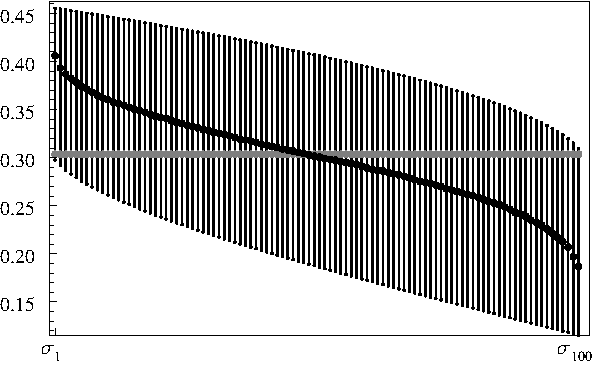
\includegraphics{col_spars_nlogn_100}
\caption{[Spectrum of a random submatrix] The matrix $\mat{U}$ is a $10^2 \times 10^4$ submatrix of the unitary DFT matrix with dimension $10^4,$ and the sampling probability $p = 10^{-4} \log(10^4).$ The $k$th vertical bar, calculated using Theorem \ref{thm:colsampling}, describes an interval containing the median value of the $k$th singular value of the sampled matrix $\widehat{\mat{U}}$. The black circles denote the empirical medians of the singular values of $\widehat{\mat{U}}$, calculated from 500 trials. The gray circles represent the singular values of $\E \widehat{\mat{U}}.$}  
\label{fig:nlogn}
\end{figure}

To illustrate the discriminatory power of these bounds, let $\mat{U}$ be an $n \times n^2$ matrix consisting of $n$ rows of the $n^2 \times n^2$ Fourier matrix and choose $p = (\log n)/n$ so that, on average, sampling reduces the aspect ratio from $n$ to $\log n.$  For $n=100,$ we determine upper and lower bounds for the median value of $\s_k(\widehat{\mat{U}})$ by numerically finding the value of $\delta$ where the probability bounds in Theorem \ref{thm:colsampling} equal $1/2.$ Figure \ref{fig:nlogn} plots the empirical median value along with the computed interval. We see that these ranges reflect the behavior of the singular values more faithfully than the simple estimates $\s_k(\mathbb{E} \widehat{\mat{U}}) = p.$

\section{Covariance Estimation}
\label{sec:covarianceest}

We conclude with an extended example that illustrates how this circle of ideas allows one to answer interesting statistical questions. Specifically, we investigate the convergence of the individual eigenvalues of sample covariance matrices, with errors measured in \emph{relative} precision.

Covariance estimation is a basic and ubiquitious problem that arises in signal processing, graphical modeling, machine learning, and genomics, among other areas. Let $\{\vec{\eta}_j\}_{j=1}^n \subset \R^p$ be i.i.d. samples drawn from some distribution with zero mean and covariance matrix $\mat{C}.$ Define the sample covariance matrix 
\[
 \widehat{\mat{C}}_n = \frac{1}{n} \sum_{j=1}^n \vec{\eta}_j\vec{\eta}_j^\star.
\]
An important challenge is to determine how many samples are needed to ensure that the empirical covariance estimator has a fixed relative accuracy in the spectral norm. That is, given a fixed $\varepsilon,$ how large must $n$ be so that 
\begin{equation}
\label{eqn:relacccovar}
 \snorm{\widehat{\mat{C}}_n - \mat{C}} \leq \varepsilon \snorm{\mat{C}}?
\end{equation}

This estimation problem has been studied extensively. It is now known that for distributions with a finite second moment, $\Omega(p \log p)$ samples suffice \cite{RU99}, and for log-concave distributions, $\Omega(p)$ samples suffice \cite{ALPT10b}. More broadly, Vershynin \cite{V10} conjectures that, for distributions with finite fourth moment, $\Omega(p)$ samples suffice; he establishes this result to within iterated log factors.

The inequality \eqref{eqn:relacccovar} ensures that the difference between the $k$th eigenvalues of $\widehat{\mat{C}}_n$ and $\mat{C}$ is small, but it measures this error on the scale of $\norm{\mat{C}}$. Therefore, the standard results on covariance estimation provide no guarantees on the relative approximation error in the $k$th eigenvalue, unless $k=1.$ In particular, condition \eqref{eqn:relacccovar} offers virtually no information on the spectrum of the estimated precision matrix $\widehat{\mat{C}}_n^{-1}.$ To obtain this information, one must measure the approximation error on the scale of $\lambdamin{\mat{C}}^{-1}.$ 

In this section, we derive a relative approximation bound for each eigenvalue of $\mat{C}.$ For simplicity we assume the samples are drawn from a $\mathcal{N}(\vec{0}, \mat{C})$ distribution where $\mat{C}$ is full-rank, but the arguments can be extended to cover other distributions.

\begin{thm}
\label{thm:covarest}
Assume that $\mat{C} \in \samats{p}$ is positive definite. Let $\{\vec{\eta}_j\}_{j=1}^n \subset \R^p$ be i.i.d. samples drawn from a $\mathcal{N}(\vec{0}, \mat{C})$ distribution. Define 
\[
\widehat{\mat{C}}_n = \frac{1}{n} \sum\nolimits_{j=1}^n \vec{\eta}_j\vec{\eta}_j^\star.
\]
Write $\lambda_k$ for the $k$th eigenvalue of $\mat{C}$, and write $\hat{\lambda}_k$ for the $k$th eigenvalue of $\widehat{\mat{C}}_n.$ Then for $k=1,\ldots,p,$
\begin{align*}
\Prob{\hat{\lambda}_k \geq \lambda_k + t} & \leq  (p-k+1) \cdot \exp\left( \displaystyle \frac{-nt^2}{32 \lambda_k \sum_{i=k}^p \lambda_i} \right) \quad \text{for } t \leq 4 n \lambda_k, \\
\intertext{ and }
\Prob{\hat{\lambda}_k \leq \lambda_k - t} & \leq  k \cdot \exp\left( \displaystyle \frac{-3nt^2}{8 \lambda_1 \big(\lambda_1 + \sum_{i=1}^k \lambda_i \big) } \right) \quad \text{for } t \leq n\big(\lambda_1 + \sum_{i=1}^k \lambda_i\big).
\end{align*}

% If $k$ is an integer in $[1,n],$ then for all $t > 0,$
% \begin{equation*}
% \Prob{\lambda_k(\hat{\mat{C}}_n) \geq \lambda_k(\mat{C}) + t} \leq 
% (p - k + 1) \cdot \exp \left( \frac{-nt^2}{\left(\sum\nolimits_{i=k}^p \lambda_i \right)(16 \lambda_k + 4t)} \right) 
% \end{equation*}
% and 
% \begin{equation*}
% \Prob{\lambda_k(\hat{\mat{C}}_n) \leq \lambda_k(\mat{C}) - t} \leq k \cdot \exp\left(\frac{-nt^2}{2 \lambda_1 \left(\lambda_1 + \sum\nolimits_{i=1}^k \lambda_i + \tfrac{t}{3} \right)} \right).
% \end{equation*}
\end{thm}

The following corollary provides an answer to our question about relative error estimates.
\begin{cor}
\label{cor:relerrcovarest}
Let $\lambda_k$ and $\hat{\lambda}_k$ be as in Theorem \ref{thm:covarest}. Then 
\begin{align*}
\Prob{\hat{\lambda}_k \geq (1 + \varepsilon) \lambda_k} & \leq 
(p-k+1) \cdot \exp\left(\frac{- c n \varepsilon^2 }{\sum\nolimits_{i=k}^p \frac{\lambda_i}{\lambda_k}} \right) \quad \text{for } \varepsilon \leq 4 n, \\
\intertext{ and }
\Prob{\hat{\lambda}_k  \leq (1 - \varepsilon) \lambda_k} & \leq k \cdot \exp\left( \frac{-c n \varepsilon^2}{\tfrac{\lambda_1}{\lambda_k}\big( \tfrac{\lambda_1}{\lambda_k} + \sum_{i=1}^k \frac{\lambda_i}{\lambda_k} \big)} \right) \quad \text{for } \varepsilon \in (0,1],
\end{align*}
where the constant $c$ is at least $1/32.$
\end{cor}

The first bound in Corollary \ref{cor:relerrcovarest} tells us how many samples are needed to ensure that $\hat{\lambda}_k$ does not overestimate $\lambda_k.$ Likewise, the second bound tells us how many samples ensure that $\hat{\lambda}_k$ does not underestimate $\lambda_k.$
%The first bound in Corollary \ref{cor:relerrcovarest} tells us how many samples are needed to ensure that $\hat{\lambda}_k$ does not appreciably overestimate $\lambda_k$. However, it is possible that with that many samples $\hat{\lambda}_k$ underestimates $\lambda_k$. Thus we say that this number of samples guarantees that $\hat{\lambda}_k$ is a \emph{robust underestimate} of $\lambda_k$: that is, $\hat{\lambda}_k$ is guaranteed to either be a genuine underestimate or to relatively overestimate $\lambda_k$ only slightly. Likewise, the second bound tells us how many samples ensure that $\hat{\lambda}_k$ does not appreciably underestimate $\lambda_k$. Since it is possible that with this many samples $\hat{\lambda}_k$ overestimates $\lambda_k$, we now interpret $\hat{\lambda}_k$ as a \emph{robust overestimate} of $\lambda_k.$ 

%Intuition suggests that one should need only a few samples to obtain an accurate upper bound on $\lambda_1$ and an accurate lower bound on $\lambda_p$. Corollary \ref{cor:relerrcovarest} quantifies this intuition, saying that $\mathrm{O}(1)$ samples are sufficient for $\hat{\lambda}_1$ and $\hat{\lambda}_p$ to be, respectively, a robust overestimate and a robust underestimate. The intuition that one needs a large number of samples to accurately upper bound $\lambda_p$ or lower bound $\lambda_1$ is also quantified: we see that $\mathrm{O}(p \log p)$ samples suffice. More generally, it follows from Corollary \ref{cor:relerrcovarest} that $\hat{\lambda}_k$ is a robust underestimate of $\lambda_k$ after $\mathrm{O}((p-k+1) \log (p-k+1) + 1)$ observations and a robust overestimate after $\mathrm{O}(k \log k + 1)$ observations. Consequently, $\mathrm{O}(p\log p)$ samples allow us to determine the full spectrum of $\mat{C}$ to within relative accuracy. 

Corollary \ref{cor:relerrcovarest} suggests that the relationship of $\hat{\lambda}_k$ to $\lambda_k$ is determined by the spectrum of $\mat{C}$ in the following natural manner. When the eigenvalues below $\lambda_k$ are small compared with $\lambda_k$, the quantity
\[
 \sum_{i=k}^p \lambda_i/\lambda_k
\]
is small, and so $\hat{\lambda}_k$ is not likely to overestimate $\lambda_k$. Similarly, when the eigenvalues above $\lambda_k$ are comparable with $\lambda_k$, the quantity
\[
\frac{\lambda_1}{\lambda_k}\left( \frac{\lambda_1}{\lambda_k} + \sum_{i=1}^k \lambda_i/\lambda_k  \right)
\]
is small, and so $\hat{\lambda}_k$ is not likely to underestimate $\lambda_k$.


% It is probably the case that a more refined analysis would find that the probability of overestimation is controlled by the ratio of \lambda_k to \lambda_{k-1} and that of underestimation is controlled by the ratio of \lambda_k to \lambda_{k+1}. I.e., only the adjacent eigenvalues affect lambda_k
% Experimentally, looks like the bound of (p \log p)/\epsilon^2 samples needed to ensure the sample covar of an indep Gaussian process has all eigenvalues within \pm\epsilon of 1 is sharp. look at bounds on wishart matrix evals for comparison (or NCK ineq)

\begin{remark}
From Corollary \ref{cor:relerrcovarest}, we see that if $n = \Omega( \varepsilon^{-2} \max \{ (p-k+1)\log(p-k+1)), k \log k \} ),$ then with high probability $\hat{\lambda}_k$ estimates $\lambda_k$ to within a relative error of $\varepsilon.$ Observe that for each of the $p$ eigenvalues, the number of samples required to ensure relative error estimation is $\mathrm{O}(\varepsilon^{-2} p \log p).$ Theorem \ref{thm:examplecovarest} now follows from a union bound.
\end{remark}

\begin{remark}
The results in Theorem \ref{thm:covarest} and Corollary \ref{cor:relerrcovarest} also apply when $\mat{C}$ is rank-deficient: simply replace each occurence of the dimension $p$ in the bounds with $\rank(\mat{C}).$ 

Indeed, assume that $\mat{C}$ is rank-deficient and take its truncated eigenvalue decomposition to be $\mat{C} = \mat{U} \mat{\Lambda} \mat{U}^\star.$ If $\vec{\eta}_j \sim \mathcal{N}(\vec{0}, \mat{C}),$ then $\vec{\eta}_j$ lies in the span of $\mat{C}.$ It follows that $\hat{\lambda}_k = \lambda_k = 0$ for all $k > \rank(\mat{C}).$ When $k \leq \rank(\mat{C}),$ we observe that  
\[
\lambda_k(\mat{C}) = \lambda_k(\mat{\Lambda}) \quad \text{ and } \quad \lambda_k\left(\sum_j \vec{\eta}_j \vec{\eta}_j^\star \right) = \lambda_k\left( \sum_j \vec{\xi}_j \vec{\xi}_j^\star \right),
\]
where $\vec{\xi}_j = \mat{U}^\star \vec{\eta}_j$ is distributed $\mathcal{N}(\vec{0}, \mat{\Lambda}).$ Thus,
\[
\left| \lambda_k\left(\sum_j \vec{\eta}_j \vec{\eta}_j^\star \right) - \lambda_k(\mat{C}) \right| =
\left| \lambda_k\left( \sum_j \vec{\xi}_j \vec{\xi}_j^\star \right) - \lambda_k(\mat{\Lambda}) \right|.
\]
Consequently, the problem of estimating the eigenvalues of $\mat{C}$ to relative error using the samples $\{\vec{\eta}_j\}$ is equivalent to that of estimating the eigenvalues of the full-rank covariance matrix $\mat{\Lambda}$ to relative error using the samples $\{\vec{\xi}_j\}.$
\end{remark}

\subsection{Proof of Theorem \ref{thm:covarest}}
We now prove Theorem \ref{thm:covarest}. This result requires a number of supporting lemmas; we defer their proofs until after a discussion of extensions to Theorem \ref{thm:covarest}.

We study the error $|\lambda_k(\widehat{\mat{C}}_n) - \lambda_k(\mat{C})|.$ To apply the methods developed in this paper, we pass to a question about the eigenvalues of a difference of two matrices. The first lemma accomplishes this goal by compressing both the population covariance matrix and the sample covariance matrix to a fixed invariant subspace of the population covariance matrix.

\begin{lemma}
\label{lemma:splittail}
Let $\mat{X}$ be a random self-adjoint matrix with dimension $p,$ and let $\mat{A}$ be a fixed self-adjoint matrix with dimension $p$. Choose $\mat{W}_+ \in \Isom{p-k+1}{p}$ and $\mat{W}_- \in \Isom{k}{p}$ for which
\[
  \lambda_k(\mat{A}) = \lambdamax{\mat{W}_+^*\mat{A}\mat{W}_+} = \lambdamin{\mat{W}_-^*\mat{A}\mat{W}_-}.
\]
Then, for all $t >0,$
\begin{align}
 \Prob{\lambda_k(\mat{X}) \geq \lambda_k(\mat{A}) + t} & \leq \Prob{\lambdamax{\mat{W}_+^\star \mat{X} \mat{W}_+} \geq \lambda_k(\mat{A}) + t } \label{eqn:covardeterministicupperbnd}\\
\intertext{ and }
 \Prob{\lambda_k(\mat{X}) \leq \lambda_k(\mat{A}) -t } &\leq \Prob{\lambdamax{\mat{W}_-^\star(\mat{A} - \mat{X}) \mat{W}_-} \geq t}.
 \label{eqn:covardeterministiclowerbnd}
\end{align}
\end{lemma}

We apply this result with $\mat{A} = \mat{C}$ and $\mat{X} = \widehat{\mat{C}}_n.$ The first estimate \eqref{eqn:covardeterministicupperbnd} and the second estimate \eqref{eqn:covardeterministiclowerbnd} are handled using different arguments. The second estimate is easier because the maximum eigenvalue of the matrix $\mat{C} - \widehat{\mat{C}}_n$ is bounded. Indeed,
\[
 \lambdamax{\mat{W}_+^\star (\mat{C} - \widehat{\mat{C}}_n) \mat{W}_+} \leq \lambdamax{\mat{W}_+^\star \mat{C} \mat{W}_+}.
\]
Thus, we may use Theorem \ref{thm:bennett} to complete the second estimate. The next lemma gives the matrix variances that we need to apply this theorem.

\begin{lemma}
\label{lemma:gaussiancentralsecondmoment}
Let $\vec{\xi} \sim \mathcal{N}(\mat{0}, \mat{G}).$ Then
$$
\E(\vec{\xi}\vec{\xi}^\star - \mat{G})^2 = \mat{G}^2 + \tr(\mat{G})\cdot \mat{G}. 
$$
\end{lemma}

The first inequality \eqref{eqn:covardeterministicupperbnd} is harder because $\widehat{\mat{C}}_n$ is unbounded. In this case, we may apply Theorem \ref{thm:subexponentialbernstein}. To use this theorem, we need the following moment growth estimate for rank-one Wishart matrices.

\begin{lemma}
\label{lemma:momentbound}
Let $\vec{\xi} \sim \mathcal{N}(\vec{0},\mat{G}).$ Then for any integer $m \geq 2,$
$$
\E\left(\vec{\xi}\vec{\xi}^\star \right)^m \preceq 2^m m! (\tr \mat{G})^{m-1}\cdot \mat{G}.
$$
\end{lemma}

With these preliminaries addressed, we prove Theorem \ref{thm:covarest}.

\begin{proof}[Proof of lower estimate]

First we consider the probability that $\hat{\lambda}_k$ underestimates $\lambda_k$. Let $\mat{W}_- \in \Isom{k}{p}$ satisfy
\[
 \lambda_k(\mat{C}) = \lambdamin{\mat{W}_-^\star \mat{C} \mat{W}_-}.
\]
Then Lemma \ref{lemma:splittail} implies
\begin{align*}
 \Prob{\lambda_k(\widehat{\mat{C}}_n) \leq \lambda_k(\mat{C}) - t} & \leq \Prob{\lambdamax{\mat{W}_-^\star (\mat{C} - \widehat{\mat{C}}_n) \mat{W}_-} \geq t} \\
& = \Prob{ \lambdamax{\sum\nolimits_j \mat{W}_-^\star(\mat{C} - \vec{\eta}_j\vec{\eta}_j^\star ) \mat{W}_-} \geq nt}.
\end{align*}
The factor $n$ comes from the normalization of the sample covariance matrix. Each term in the sum is zero mean and bounded above by $\mat{W}_-^*\mat{C}\mat{W}_-$ in the semidefinite order, so Theorem \ref{thm:bennett} applies. As we desire a bound on the maximum eigenvalue of the sum, we take $\mat{V}_+ = \mathbf{I}$ when we invoke Theorem \ref{thm:bennett}. Then 
\[
 \sigma_1^2 = \lambdamax{ \sum\nolimits_j \E\left[\mat{W}_-^\star(\mat{C} - \vec{\eta}_j\vec{\eta}_j^\star)\mat{W}_-\right]^2 } = n \lambdamax{\E\left[\mat{W}_-^\star(\mat{C} - \vec{\eta}_1\vec{\eta}_1^\star)\mat{W}_-\right]^2}.
\]
The covariance matrix of $\vec{\eta}_1$ is $\mat{C},$ so that of $\mat{W}_-^\star \vec{\eta}_1$ is $\mat{W}_-^\star \mat{C} \mat{W}_-.$ It follows from  Lemma \ref{lemma:gaussiancentralsecondmoment} that
\[
\E\left[\mat{W}_-^*(\mat{C} - \vec{\eta}_1\vec{\eta}_1^\star)\mat{W}_-\right]^2 = (\mat{W}_-^*\mat{C}\mat{W}_-)^2 + \tr(\mat{W}_-^*\mat{C}\mat{W}_-) \cdot \mat{W}_-^*\mat{C}\mat{W}_-.
\]
Observe that $\mat{W}_-^*\mat{C}\mat{W}_-$ is the restriction of $\mat{C}$ to its dominant $k$-dimensional invariant subspace, so
\[
 \sigma_1^2 = n \lambdamax{\E\left[\mat{W}_-^\star(\mat{C} - \vec{\eta}_1\vec{\eta}_1^\star)\mat{W}_-\right]^2} = n\lambda_1(\mat{C}) \big( \lambda_1(\mat{C}) + \sum_{i=1}^k \lambda_i(\mat{C}) \big) 
\]
and we can take $\randcon(\mat{V}_+) = \lambdamax{\mat{C}}.$

The subgaussian branch of the split Bernstein inequality of Theorem \ref{thm:bennett} shows that 
\begin{equation*}
 \Prob{ \lambdamax{\sum\nolimits_j \mat{W}_-^\star(\mat{C} - \vec{\eta}_j\vec{\eta}_j^\star ) \mat{W}_-} \geq nt} \leq 
 k \cdot \exp\left( \displaystyle \frac{-3nt^2}{8 \lambda_1(\mat{C}) \big(\lambda_1(\mat{C}) + \sum_{i=1}^k \lambda_i(\mat{C}) \big) } \right)
\end{equation*}
when  $t \leq n\big(\lambda_1(\mat{C}) + \sum_{i=1}^k \lambda_i(\mat{C})\big).$ This inequality provides the desired bound on the probability that $\lambda_k(\widehat{\mat{C}}_n)$ underestimates $\lambda_k(\mat{C})$.
\end{proof}

\begin{proof}[Proof of upper estimate]
Now we consider the probability that $\hat{\lambda}_k$ overestimates $\lambda_k$. Let $\mat{W}_+ \in \Isom{p-k+1}{p}$ satisfy
\[
 \lambda_k(\mat{C}) = \lambdamax{\mat{W}_+^\star \mat{C} \mat{W}_+}.
\]
Then Lemma \ref{lemma:splittail} implies
\begin{align}
 \Prob{\lambda_k(\widehat{\mat{C}}_n) \geq \lambda_k(\mat{C}) + t} & \leq \Prob{\lambdamax{\mat{W}_+^\star \widehat{\mat{C}}_n \mat{W}_+} \geq \lambda_k(\mat{C}) + t} \notag \\
& = \Prob{\lambdamax{\sum\nolimits_j \mat{W}_+^\star (\vec{\eta}_j \vec{\eta}_j^\star) \mat{W}_+} \geq n \lambda_k(\mat{C}) + n t}.
\label{eqn:upperestimateprob}
\end{align}
The factor $n$ comes from the normalization of the sample covariance matrix.

The covariance matrix of $\vec{\eta}_j$ is $\mat{C},$ so that of $\mat{W}_+^\star \vec{\eta}_j$ is $\mat{W}_+^\star\mat{C}\mat{W}_+.$ Apply Lemma \ref{lemma:momentbound} to verify that $\mat{W}_+^\star \vec{\eta}_j$ satisfies the subexponential moment growth bound required by Theorem \ref{thm:subexponentialbernstein} with 
\[
 B = 2 \tr(\mat{W}_+^*\mat{C}\mat{W}_+) \quad\text{ and }\quad \mat{\Sigma}_j^2 = 8\tr(\mat{W}_+^*\mat{C}\mat{W})\cdot \mat{W}_+^*\mat{C}\mat{W}_+.
\]
In fact, $\mat{W}_+^*\mat{C}\mat{W}_+$ is the compression of $\mat{C}$ to the invariant subspace corresponding with its bottom $p-k+1$ eigenvalues, so 
\[
B = 2 \sum\nolimits_{i=k}^p \lambda_i(\mat{C}) \quad\text{and}\quad \lambdamax{\mat{\Sigma}_j^2} = 8 \lambda_k(\mat{C}) \sum\nolimits_{i=k}^p \lambda_i(\mat{C}).
\]
We are concerned with the maximum eigenvalue of the sum in \eqref{eqn:upperestimateprob}, so we take $\mat{V}_+ = \mathbf{I}$ in the statement of Theorem \ref{thm:subexponentialbernstein} to find that
\begin{align*}
 \sigma_1^2 & = \lambdamax{\sum\nolimits_j \mat{\Sigma}_j^2 } = n \lambdamax{\mat{\Sigma}_1^2} = 8 n \lambda_k(\mat{C}) \sum\nolimits_{i=k}^p \lambda_i(\mat{C}) \quad \text{and}
\\ \mu_1 & = \lambdamax{\sum_j \mat{W}_+^\star \E(\vec{\eta}_j\vec{\eta}_j^\star) \mat{W}_+ } = n\lambdamax{\mat{W}_+^\star \mat{C} \mat{W}_+} = n \lambda_k(\mat{C}).
\end{align*}
It follows from the subgaussian branch of the split Bernstein inequality of Theorem \ref{thm:subexponentialbernstein} that 
$$
\Prob{\lambda_k \left(\sum\nolimits_j \mat{W}_+^\star (\vec{\eta}_j \vec{\eta}_j^\star) \mat{W}_+ \right) \geq n \lambda_k(\mat{C}) + n t} \leq 
 (p-k+1) \cdot \exp\left( \displaystyle \frac{-nt^2}{32 \lambda_k(\mat{C}) \sum_{i=k}^p \lambda_i(\mat{C})} \right)
$$
when $t \leq 4 n \lambda_k(\mat{C}).$ This provides the desired bound on the probability that $\lambda_k(\widehat{\mat{C}}_n)$ overestimates $\lambda_k(\mat{C}).$
\end{proof}



\subsection{Extensions of Theorem \ref{thm:covarest}}
Results analogous to Theorem \ref{thm:covarest} can be established for other distributions. If the distribution is bounded, the possibility that $\hat{\lambda}_k$ deviates above or below $\lambda_k$ can be controlled using the Bernstein inequality of Theorem \ref{thm:bennett}. If the distribution is unbounded but has matrix moments that satisfy a sufficiently nice growth condition, the probability that $\hat{\lambda}_k$ deviates below $\lambda_k$ can be controlled with the Bernstein inequality of Theorem \ref{thm:bennett} and the probability that it deviates above $\lambda_k$ can be bounded using a Bernstein inequality analogous to that in Theorem \ref{thm:subexponentialbernstein}.

We established Theorem \ref{thm:covarest} using this technique to demonstrate the simplicity of the Laplace transform machinery. However, the results of \cite{ALPT10b} on the convergence of empirical covariance matrices of isotropic log-concave random vectors lead to tighter bounds on the probability that $\hat{\lambda}_k$ overestimates $\lambda_k.$ There does not seem to be an analogous reduction for handling the probability that $\hat{\lambda}_k$ is an underestimate.

To see the relevance of the results in \cite{ALPT10b}, first observe the following consequence of the subadditivity of the maximum eigenvalue mapping:
\begin{align*}
\lambdamax{\mat{W}_+^\star(\mat{X} - \mat{A}) \mat{W}_+} & \geq \lambdamax{\mat{W}_+^\star \mat{X} \mat{W}_+} - \lambdamax{\mat{W}_+^\star \mat{A} \mat{W}_+} \\
 &= \lambdamax{\mat{W}_+^\star \mat{X} \mat{W}_+} - \lambda_k(\mat{A}).
\end{align*}
In conjunction with \eqref{eqn:covardeterministicupperbnd}, this gives us the following control on the probability that $\lambda_k(\mat{X})$ overestimates $\lambda_k(\mat{A}):$ 
\[
 \Prob{\lambda_k(\mat{X}) \geq \lambda_k(\mat{A}) + t} \leq \Prob{\lambdamax{\mat{W}_+^\star (\mat{X} - \mat{A}) \mat{W}_+} \geq t}.
\]

In our application, $\mat{X}$ is the empirical covariance matrix and $\mat{A}$ is the actual covariance matrix. The spectral norm dominates the maximum eigenvalue, so 
\begin{align*}
 \Prob{\lambda_k(\widehat{\mat{C}}_n) \geq \lambda_k(\mat{C}) + t} & \leq \Prob{\lambdamax{\mat{W}_+^\star(\widehat{\mat{C}}_n - \mat{C})\mat{W}_+} \geq t}\\
& \leq \Prob{\|\mat{W}_+^\star (\widehat{\mat{C}}_n - \mat{C}) \mat{W}_+\| \geq t} = \Prob{\|\mat{W}_+^\star \widehat{\mat{C}}_n \mat{W}_+ - \mat{S}^2 \| \geq t },
\end{align*}
where $\mat{S}$ is the square root of $\mat{W}_+^\star \mat{C} \mat{W}_+.$ Now factor out $\mat{S}^2$ and identify $\lambda_k(\mat{C}) = \|\mat{S}^2\|$ to obtain
\begin{align*}
 \Prob{\lambda_k(\widehat{\mat{C}}) \geq \lambda_k(\mat{C}) + t} & \leq \Prob{\|\mat{S}^{-1} \mat{W}_+^\star \widehat{\mat{C}}_n \mat{W}_+ \mat{S}^{-1} - \mathbf{I} \| \|\mat{S}^2\| \geq t } \\
 & = \Prob{\|\mat{S}^{-1} \mat{W}_+^\star \widehat{\mat{C}}_n \mat{W}_+ \mat{S}^{-1} - \mathbf{I} \| \geq t/\lambda_k(\mat{C})}.
\end{align*}
Note that if $\vec{\eta}$ is drawn from a $\mathcal{N}(\vec{0}, \mat{C})$ distribution, then the covariance matrix of the transformed sample $\mat{S}^{-1}\mat{W}_+^\star \vec{\eta}$ is the identity:
\[
\E \left(\mat{S}^{-1}\mat{W}_+^\star \vec{\eta} \vec{\eta}^\star \mat{W}_+ \mat{S}^{-1}\right) = \mat{S}^{-1} \mat{W}_+^\star \mat{C} \mat{W}_+ \mat{S}^{-1} = \mathbf{I}.
\]
Thus $\mat{S}^{-1} \mat{W}_+^\star \widehat{\mat{C}}_n \mat{W}_+ \mat{S}^{-1}$ is the empirical covariance matrix of a standard Gaussian vector in $\R^{p-k+1}.$ By Theorem 1 of \cite{ALPT10b}, it follows that $\hat{\lambda}_k$ is unlikely to overestimate $\lambda_k$ in relative error when the number $n$ of samples is $\Omega(p-k+1).$

Similarly, for more general distributions, the bounds on the probability of $\hat{\lambda}_k$ exceeding $\lambda_k$ can be tightened beyond those suggested in Theorem \ref{thm:covarest} by using the results in \cite{ALPT10b} or \cite{V10}.

Finally, we note that the techniques developed in the proof of Theorem \ref{thm:covarest} can be used to investigate the spectrum of the error matrices $\widehat{\mat{C}}_n - \mat{C}.$
\subsection{Proofs of the supporting lemmas}

We now establish the lemmas used in the proof of Theorem \ref{thm:covarest}.

\begin{proof}[Proof of Lemma \ref{lemma:splittail}]
The probability that $\lambda_k(\mat{X})$ overestimates $\lambda_k(\mat{A})$ is controlled with the sequence of inequalities
\begin{align*}
\Prob{\lambda_k(\mat{X}) \geq \lambda_k(\mat{A}) + t} & = \Prob{ \inf_{\mat{W} \in \Isom{p-k+1}{p}} \lambdamax{\mat{W}^*\mat{X}\mat{W}} \geq \lambda_k(\mat{A}) + t} \\
& \leq \Prob{\lambdamax{\mat{W}_+^*\mat{X}\mat{W}_+} \geq \lambda_k(\mat{A}) + t}. 
\end{align*}

We use a related approach to study the probability that $\lambda_k(\mat{X})$ underestimates $\lambda_k(\mat{A}).$ Our choice of $\mat{W}_-$ implies that 
\[
\lambda_{p-k+1}(-\mat{A}) = -\lambda_k(\mat{A}) = -\lambdamin{\mat{W}_-^*\mat{A}\mat{W}_-} = \lambdamax{\mat{W}_-^*(-\mat{A})\mat{W}_-}. 
\]
It follows that
\begin{align*}
\Prob{\lambda_k(\mat{X}) \leq \lambda_k(\mat{A}) - t} & = \Prob{\lambda_{p-k+1}(-\mat{X}) \geq \lambda_{p-k+1}(-\mat{A}) + t} \\
& = \Prob{ \inf_{\mat{W} \in \Isom{k}{p}} \lambdamax{\mat{W}^*(-\mat{X})\mat{W}} \geq \lambdamax{\mat{W}_-^*(-\mat{A})\mat{W}_-} + t} \\
& \leq \Prob{\lambdamax{\mat{W}_-^*(-\mat{X})\mat{W}_-} - \lambdamax{\mat{W}_-^*(-\mat{A})\mat{W}_-} \geq t} \\
& \leq \Prob{\lambdamax{\mat{W}_-^*(\mat{A} - \mat{X})\mat{W}_-} \geq t}. 
\end{align*}
The final inequality follows from the subadditivity of the maximum eigenvalue mapping. 

This establishes the bounds on the probabilities of $\lambda_k(\mat{X})$ deviating above or below $\lambda_k(\mat{A}).$
\end{proof}

\begin{proof}[Proof of Lemma \ref{lemma:gaussiancentralsecondmoment}]
We begin by taking $\mat{S}$ to be the positive-semidefinite square root of $\mat{G}.$ Let $\mat{S} = \mat{U} \mat{\Lambda} \mat{U}^\star$ be the eigenvalue decomposition of $\mat{S},$ and let $\vec{\gamma}$ be a $\mathcal{N}(\vec{0}, \mathbf{I}_p)$ random variable. Recalling that $\mat{G}$ is the covariance matrix of $\mat{\xi}$, we see that $\vec{\xi}$ and $\mat{U} \mat{\Lambda} \vec{\gamma}$ are identically distributed. Thus,
\begin{align}
\E(\vec{\xi}\vec{\xi}^\star - \mat{G})^2 
& = \E(\mat{U} \mat{\Lambda} \vec{\gamma}\vec{\gamma}^\star \mat{\Lambda} \mat{U}^\star - \mat{U} \mat{\Lambda}^2 \mat{U}^\star)^2 \notag \\
& = \mat{U} \mat{\Lambda} \E(\vec{\gamma}\vec{\gamma}^\star \mat{\Lambda}^2 \vec{\gamma}\vec{\gamma}^\star) \mat{\Lambda} \mat{U}^\star - \mat{G}^2. 
\label{eqn:rankonewishartmatrixvarianceexpansion}
\end{align}

Consider the $(i,j)$ entry of the matrix being averaged:
\[
\E(\vec{\gamma}\vec{\gamma}^\star \mat{\Lambda}^2 \vec{\gamma}\vec{\gamma}^\star)_{ij} =  \sum_k \E(\gamma_i \gamma_j \gamma_k^2) \lambda_k^2.
\]
The $(i,j)$ entry of this matrix is zero because the entries of $\vec{\gamma}$ are independent and symmetric. Furthermore, the $(i,i)$ entry satisfies
\[
\E(\vec{\gamma}\vec{\gamma}^\star \mat{\Lambda}^2 \vec{\gamma}\vec{\gamma}^\star)_{ii} = \E(\gamma_i^4) \lambda_i^2 + \sum_{k \neq i} \E(\gamma_k^2) \lambda_k^2 = 2 \lambda_i^2 + \tr(\mat{\Lambda}^2).
\]
We have shown
\[
\E(\vec{\gamma} \vec{\gamma}^\star \mat{\Lambda}^2 \vec{\gamma}\vec{\gamma}^\star) = 2 \mat{\Lambda}^2 + \tr(\mat{G}) \cdot \mathbf{I}.
\]
This equality and \eqref{eqn:rankonewishartmatrixvarianceexpansion} imply the desired result.
\end{proof}

%\begin{proof}[Proof of Lemma \ref{lemma:gaussiancentralsecondmoment}]
%We begin by taking $\mat{G}$ to be the positive-semidefinite square root of $\mat{C}.$ Let $\vec{\gamma}$ be a $\mathcal{N}(\vec{0},\mathbf{I})$ random variable. Recalling that $\vec{\xi} \sim \mathcal{N}(\vec{0}, \mat{C}),$ we see that $\vec{\xi}$ and $\mat{G}\vec{\gamma}$ are identically distributed, so 
%\begin{align*} 
%\E(\vec{\xi}\vec{\xi}^\star - \mat{C})^2 & 
%= \E(\mat{G}(\vec{\gamma}\vec{\gamma}^\star - \mathbf{I})\mat{G})^2 
%= \mat{G} \E (\vec{\gamma}\vec{\gamma}^\star \mat{G}^2 \vec{\gamma}\vec{\gamma}^\star) \mat{G} - \mat{G}^4. 
%\end{align*}
%Next, consider the $(i,j)$ entry of the matrix being averaged:
%$$
%(\vec{\gamma}\vec{\gamma}^\star \mat{G}^2 \vec{\gamma}\vec{\gamma}^\star)_{ij} = \sum_{kl} \gamma_i \gamma_j \gamma_k \gamma_l (\mat{G}^2)_{ij}. 
%$$
%Using the properties of standard Gaussian variables,
%$$
%\E (\gamma_i \gamma_j \gamma_k \gamma_l) = 
%\begin{cases}
%1 & \text{ if } i=j, k=l, i\neq k \\
%1 & \text{ if } i=k, j=l, i \neq j \\
%1 & \text{ if } i=l, j=k, i \neq j \\
%3 & \text{ if } i= j = k= l \\
%0 & \text{ otherwise, }
%\end{cases}
%$$
%so the $(i,j)$ entry of the matrix under consideration is
%$$
%(\vec{\gamma}\vec{\gamma}^\star \mat{G}^2 \vec{\gamma}\vec{\gamma}^\star)_{ij} = \delta_{ij} \left[ 3 (\mat{G}^2)_{ij} + \sum_{k \neq i} (\mat{G}^2)_{kk} \right] + (1 - \delta_{ij})[ (\mat{G}^2)_{ij} + (\mat{G}^2)_{ji} ] = 2 (\mat{G}^2)_{ij} + \tr \mat{G}^2.
%$$
%Therefore, 
%\begin{align*} 
%\E(\vec{\xi}\vec{\xi}^\star - \mat{C})^2 
%= \mat{G} \E (\vec{\gamma}\vec{\gamma}^\star \mat{G}^2 \vec{\gamma}\vec{\gamma}^\star) \mat{G} - \mat{G}^4 = \mat{C}^2 + \tr(\mat{C}) \mat{C}.
%\end{align*}
%This is the desired expression for the matrix variance of a rank-one Wishart matrix.
%\end{proof}

\begin{proof}[Proof of Lemma \ref{lemma:momentbound}]

Factor the covariance matrix of $\vec{\xi}$ as $\mat{G} = \mat{U\Lambda U}^\star$ where $\mat{U}$ is orthogonal and $\mat{\Lambda} = \text{diag}(\lambda_1, \ldots, \lambda_p)$ is the matrix of eigenvalues of $\mat{G}$. Let $\vec{\gamma}$ be a $\mathcal{N}(\vec{0},\mathbf{I}_p)$ random variable. Then $\vec{\xi}$ and $\mat{U\Lambda}^{1/2} \vec{\gamma}$ are identically distributed, so 
\begin{align} 
\E (\vec{\xi}\vec{\xi}^\star)^m & = \E\left[(\vec{\xi}^\star\vec{\xi})^{m-1} \vec{\xi}\vec{\xi}^\star \right] = \E\left[ (\vec{\gamma}^\star \mat{\Lambda} \vec{\gamma})^{m-1} \mat{U\Lambda}^{1/2} \vec{\gamma}\vec{\gamma}^\star \mat{\Lambda}^{1/2} \mat{U}^\star \right]\notag \\
 & = \mat{U\Lambda}^{1/2} \E \left[ (\vec{\gamma}^\star \mat{\Lambda} \vec{\gamma})^{m-1} \vec{\gamma}\vec{\gamma}^\star \right] \mat{\Lambda}^{1/2}\mat{U}^\star. 
\label{eqn:rankonewishartpowers}
\end{align}
Consider the $(i,j)$ entry of the bracketed matrix in \eqref{eqn:rankonewishartpowers}:
\begin{equation}
\E\left[(\vec{\gamma}^\star \mat{\Lambda} \vec{\gamma})^{m-1} \gamma_i\gamma_j \right] = \E\left[\left(\sum\nolimits_{\ell=1}^p \lambda_\ell \gamma_\ell^2 \right)^{m-1} \gamma_i \gamma_j\right]. 
\label{eqn:gaussianchaos}
\end{equation}
From this expression, and the independence of the Gaussian variables $\{ \gamma_i \},$ we see that this matrix is diagonal.

To bound the diagonal entries, use a multinomial expansion to further develop the sum in \eqref{eqn:gaussianchaos} for the $(i,i)$ entry:
\[
 \E\left[(\vec{\gamma}^\star \mat{\Lambda} \vec{\gamma})^{m-1} \gamma_i^2 \right]  
= \sum_{\ell_1 + \cdots +\ell_p = m-1} \left({m-1 \atop \ell_1, \ldots, \ell_p } \right) \lambda_1^{\ell_1} \cdots \lambda_p^{\ell_p} \E\left[\gamma_1^{2\ell_1} \cdots \gamma_p^{2\ell_p} \gamma_i^2 \right].
\]
%Now we use the generalized AM--GM inequality to replace the expectation of the product of Gaussians with the $2m$th moment of a single standard Gaussian $g$. 
Denote the $L_r$ norm of a random variable $X$ by
\[ 
  \lnorm{r}{X} = \left(\E |X|^r \right)^{1/r}. 
\]
Since $\ell_1, \ldots, \ell_p$ are nonnegative integers summing to $m-1$, the generalized AM-GM inequality justifies the first of the following inequalities:
\begin{align*}
\E \gamma_1^{2\ell_1} \cdots \gamma_p^{2\ell_p} \gamma_i^2 & \leq  \E \left(\frac{\ell_1 |\gamma_1| + \cdots + \ell_p |\gamma_p| + |\gamma_i|}{m}\right)^{2m} =
 \lnorm{2m}{ \frac{1}{m} \left(|\gamma_i| + \sum_{j=1}^p \ell_j |\gamma_j| \right) }^{2m} \\
 & \leq \left( \frac{1}{m} \left( \lnorm{2m}{\gamma_i} + \sum_{j=1}^p \ell_j \lnorm{2m}{\gamma_j} \right) \right)^{2m} \\
 & = \left(\frac{1 + \ell_1 + \ldots + \ell_p}{m} \right)^{2m} \lnorm{2m}{g}^{2m} = \E (g^{2m}).  
\end{align*}
The second inequality is the triangle inequality for $L_r$ norms. Now we reverse the multinomial expansion to see that the diagonal terms satisfy the inequality
\begin{align}
\E\left[(\vec{\gamma}^\star \mat{\Lambda} \vec{\gamma})^{m-1}\gamma_i^2\right] & \leq \sum_{\ell_1 + \cdots + \ell_p = m-1} \left({ m-1 \atop \ell_1, \ldots, \ell_p }\right) \lambda_1^{\ell_1} \cdots \lambda_p^{\ell_p} \E (g^{2m}) \notag \\
&  = (\lambda_1 + \ldots + \lambda_p)^{m-1}\E ( g^{2m}) = \tr(\mat{G})^{m-1} \E (g^{2m}). 
\label{eqn:diagonalest}
\end{align}
Estimate $\E(g^{2m})$ using the fact that $\Gamma(x)$ is increasing for $x \geq 1:$
\begin{align*}
\E \left( g^{2m} \right) & = \frac{2^m}{\sqrt{\pi}} \Gamma(m + 1/2) < \frac{2^m}{\sqrt{\pi}} \Gamma(m+1) = \frac{2^m}{\sqrt{\pi}} m! \quad \text{for } m \geq 1.
\end{align*}
Combine this result with \eqref{eqn:diagonalest} to see that
\[
\E\left[(\vec{\gamma}^\star \mat{\Lambda} \vec{\gamma})^{m-1}\vec{\gamma}\vec{\gamma}^\star \right] \preceq \frac{2^m}{\sqrt{\pi}} m! \tr(\mat{G})^{m-1} \cdot \mathbf{I}. 
\] 
Complete the proof by using this estimate in \eqref{eqn:rankonewishartpowers}.
%\begin{equation}
%\E (\vec{\xi}\vec{\xi}^\star)^m \preceq \mat{U\Lambda}^{1/2}\tr(\mat{G})^{m-1} \left(\frac{2^m}{\sqrt{\pi}} m! \cdot \mathbf{I} \right) \mat{\Lambda}^{1/2}\mat{U}^\star \preceq 2^m m! (\tr \mat{G})^{m-1} \mat{G}. 
%\end{equation}

\end{proof}

% \begin{lemma}
% \label{lemma:bernsteinmomentbound}
% Let $\mat{X}$ be a random $n \times n$ self-adjoint matrix such that for some positive semidefinite $\mat{\sigma}^2$ and some constant $M \in (0, \infty),$
% \begin{equation}
% \E \mat{X}^k \preceq \frac{k!}{2} \mat{\sigma}^2 M^{k-2} \quad \text{for } k \geq 2. 
% \label{eqn:bernsteinmomentbound}
% \end{equation}
% Then 
% $$
% \E \exp(\theta \mat{X}) \preceq \exp\left(\theta \E\mat{X} + \frac{\theta^2 \mat{\sigma}^2}{2-2M\theta}\right) \quad \text{for } 0 \leq M\theta < 1.
% $$
% \end{lemma}


\bibliographystyle{amsalpha}
\bibliography{minimax_matrix_laplace_transform}
\end{document}
